%%%%%%%%%%%%%%%%%%%%%%%%%%%%%%%%%%%%%%%%%%%%%%%%%%%%%%%%%%%%%%%%%%%%%%%%%%%%%%%

%
% TODO:
% * Zhou or Quinn: what is the SpType? Add to abstract, tables, and
% text. G0V has been assumed.
%

\documentclass[12pt,twocolumn,tighten]{aastex63}
%\documentclass[12pt,twocolumn,tighten,trackchanges]{aastex63}
\usepackage{amsmath,amstext,amssymb}
\usepackage[T1]{fontenc}
\usepackage{apjfonts}
\usepackage[figure,figure*]{hypcap}
\usepackage{graphics,graphicx}
\usepackage{hyperref}
\usepackage{natbib}
\usepackage[caption=false]{subfig} % for subfloat
\usepackage{enumitem} % for specific spacing of enumerate
\usepackage{epigraph}

\renewcommand*{\sectionautorefname}{Section} %for \autoref
\renewcommand*{\subsectionautorefname}{Section} %for \autoref

\newcommand{\tn}{TOI~837} % target star name
\newcommand{\pn}{TOI~837.01} % planet name
\newcommand{\cn}{IC~2602} % cluster name

\newcommand{\kms}{\,km\,s$^{-1}$}

\newcommand{\stscilink}{\textsc{\url{archive.stsci.edu/hlsp/cdips}}}
\newcommand{\datasetlink}{\textsc{\dataset[doi.org/10.17909/t9-ayd0-k727]{https://doi.org/10.17909/t9-ayd0-k727}}}

%% Reintroduced the \received and \accepted commands from AASTeX v5.2.
%% Add "Submitted to " argument.
\received{\today}
\revised{---}
\accepted{---}
\submitjournal{AAS journals.}
\shorttitle{TOI~837 in IC~2602}

\begin{document}

\defcitealias{bouma_wasp4b_2019}{B19}

\title{
  Cluster Difference Imaging Photometric Survey (CDIPS) II.
  TOI$\,$837: A Validated Jupiter-Sized Planet in IC~2602
}

\suppressAffiliations
%\NewPageAfterKeywords
\correspondingauthor{L.\,G.\,Bouma}
\email{luke@astro.princeton.edu}

%
% key authors:
%

\author[0000-0002-0514-5538]{L. G. Bouma}
\affiliation{Department of Astrophysical Sciences, Princeton
University, 4 Ivy Lane, Princeton, NJ 08540, USA}

%PENDING
\author[0000-0002-9158-7315]{R. Brahm}
\affiliation{Center of Astro-Engineering UC, Pontificia Universidad
Cat\'olica de Chile, Av. Vicu\~na Mackenna 4860, 782-0436 Macul,
Santiago, Chile}
\affiliation{Instituto de Astrof\'isica, Facultad de F\'isica,
Pontificia Universidad Cat\'olica de Chile, Av. Vicu\~na Mackenna
4860, 782-0436 Macul, Santiago, Chile}
\affiliation{Millennium Institute of Astrophysics, Av. Vicu\~na
Mackenna 4860, 782-0436 Macul, Santiago, Chile}

\author[0000-0001-8732-6166]{J. D. Hartman}
\affiliation{Department of Astrophysical Sciences, Princeton
University, 4 Ivy Lane, Princeton, NJ 08540, USA}

%PENDING
\author{J. de Leon}
\affiliation{Department of Astronomy, University of Tokyo, 7-3-1
Hongo, Bunkyo-ky, Tokyo 113-0033, Japan}

%
% SG1 contributors: ask Karen -- are there others?
%
%PENDING
\author{P. Evans}
\affiliation{El Sauce Observatory, Coquimbo Province, Chile}

%PENDING
\author[0000-0001-6588-9574]{K. A. Collins} % karenacollins@outlook.com
\affiliation{Center for Astrophysics \textbar \ Harvard \&
Smithsonian, 60 Garden St, Cambridge, MA 02138, USA}

%
% SG2 contributors
%
%PENDING
\author[0000-0002-4891-3517]{G. Zhou}
\affiliation{Center for Astrophysics \textbar \ Harvard \&
Smithsonian, 60 Garden St, Cambridge, MA 02138, USA}

%PENDING
\author[0000-0002-8964-8377]{S. N. Quinn} % squinn@cfa.harvard.edu
\affiliation{Center for Astrophysics \textbar \ Harvard \&
Smithsonian, 60 Garden St, Cambridge, MA 02138, USA}

%
% SG4 contributors
%
\author[0000-0002-0619-7639]{C.~Ziegler}
\affiliation{Dunlap Institute for Astronomy and Astrophysics,
University of Toronto, 50 St. George Street, Toronto, Ontario M5S 3H4,
Canada}

%
% UToyko team
%
%PENDING
\author[0000-0002-4881-3620]{J. Livingston}
\affiliation{Department of Astronomy, University of Tokyo, 7-3-1
Hongo, Bunkyo-ky, Tokyo 113-0033, Japan}

%
% MPIA team
%
%PENDING
\author{T. Henning}
\affiliation{Max-Planck-Institut f\"ur Astronomie, K\"onigstuhl 17,
69117 Heidelberg, Germany}

%PENDING
\author[0000-0002-5389-3944]{A. Jord\'an}
\affiliation{Facultad de Ingenier\'ia y Ciencias, Universidad Adolfo
Ib\'a\~nez, Av.\ Diagonal las Torres 2640, Pe\~nalol\'en, Santiago,
Chile}
\affiliation{Millennium Institute of Astrophysics, Av. Vicu\~na
Mackenna 4860, 782-0436 Macul, Santiago, Chile}

%PENDING
\author[0000-0001-9513-1449]{N. Espinoza}
\affil{Space Telescope Science Institute, 3700 San Martin Drive,
Baltimore, MD 21218, USA}


%
% Princeton team
%
%PENDING
\author[0000-0002-0628-0088]{W. Bhatti}
\affiliation{Department of Astrophysical Sciences, Princeton
University, 4 Ivy Lane, Princeton, NJ 08540, USA}
%
\author[0000-0002-4265-047X]{J. N. Winn}
\affiliation{Department of Astrophysical Sciences, Princeton
University, 4 Ivy Lane, Princeton, NJ 08540, USA}
%
\author[0000-0001-7204-6727]{G. \'A. Bakos}
\affiliation{Department of Astrophysical Sciences, Princeton
University, 4 Ivy Lane, Princeton, NJ 08540, USA}

% 
%-------------------------------------
% TESS Mission Architects:
% These authors should be listed in this order
% see https://spacebook.mit.edu/pages/viewpage.action?pageId=24543276
%-------------------------------------
%
%CONFIRMED
\author{G. R. Ricker} % grr@space.mit.edu
\affiliation{Department of Physics and Kavli Institute for Astrophysics
and Space Research, Massachusetts Institute of Technology, Cambridge, MA
02139, USA}
%
%PENDING
\author[0000-0001-6763-6562]{R. Vanderspek} % roland@space.mit.edu
\affiliation{Department of Physics and Kavli Institute for Astrophysics
and Space Research, Massachusetts Institute of Technology, Cambridge, MA
02139, USA}
%
%CONFIRMED
\author[0000-0001-9911-7388]{D. W.~Latham} % dlatham@cfa.harvard.edu
\affiliation{Center for Astrophysics \textbar \ Harvard \&
Smithsonian, 60 Garden St, Cambridge, MA 02138, USA}
%
%PENDING
\author{S. Seager} % seager@mit.edu
\affiliation{Department of Earth, Atmospheric, and Planetary Sciences,
Massachusetts Institute of Technology, Cambridge, MA 02139, USA}
%
%PENDING
\author[0000-0002-4715-9460]{J. M.~Jenkins} % jon.jenkins@nasa.gov
\affiliation{NASA Ames Research Center, Moffett Field, CA 94035, USA}
%
%-------------------------------------
% 3 representatives of each of SPOC, POC, TSO, for a total of 9. 
%These 9 authors should be listed in alphabetical order
%-------------------------------------
% 3 TSO COAUTHORS
%     Karen Collins karenacollins@outlook.com
%     Sam Quinn squinn@cfa.harvard.edu
%     Dana Louie danalouie@astro.umd.edu
% 3 SPOC COAUTHORS
%     Mark E. Rose mark.rose@nasa.gov
%     Jeffrey C. Smith  jeffrey.c.smith-1@nasa.gov
%     Bill Wohler  bill.wohler@nasa.gov
% 3 POC COAUTHORS: 
%     John Doty (jpd@noqsi.com)
%     Joel Villaseñor (jsvilla@space.mit.edu)
%     Tom Barclay (barclay.astro@gmail.com)

\author{TSO/SPOC/POC representatives}





\begin{abstract}
  We report the discovery of TOI 837.01 and its validation as a
  transiting planet.  We characterize the system using data from the
  NASA TESS mission, the ESA Gaia mission, ground-based photometry,
  and spectroscopy from CHIRON, FEROS, and Veloce.  We find that
  TOI$\,$837 is a $T=9.9$ G0 dwarf in IC 2602.  The star and validated
  planet are therefore between 30 and 46 million years old.  The
  planet is warm ($P = 8.32\,{\rm d}$) and roughly Jupiter-sized.
  However, its transits are grazing: $b > 0.92$ at 3$\sigma$.  From
  TESS photometry alone, the planetary size lies within 0.58--3.87
  $R_{\rm Jup}$ (3$^{\rm rd}$--97$^{\rm th}$ percentile), due to the
  degeneracy between the planetary size and the impact parameter of
  the transit.  From radial velocity monitoring, we limit the minimum
  mass to less than 1.20 $M_{\rm Jup}$ (3$\sigma$).  Grazing transits
  are cause for concern: they usually are indicative of astrophysical
  false positive scenarios.  Our follow-up data show that such
  scenarios are highly unlikely.  Multi-color photometry requires
  eclipsing companions to have nearly identical color as TOI$\,$837,
  ruling out hierarchical eclipsing binary scenarios.  Background
  eclipsing binary scenarios are limited by speckle imaging, but
  formally remain a 0.2\% possibility.  TOI 837.01 is therefore a
  validated adolescent exoplanet.  Further observations of its stellar
  obliquity, atmosphere, and mass should confirm its planetary nature
  beyond doubt, and could improve our understanding of how the
  physical and orbital properties of exoplanets change in time.
\end{abstract}

\keywords{
	Exoplanets (498),
  Transits (1711),
	Exoplanet evolution (491),
	Stellar ages (1581),
	Young star clusters (1833)
}

%%%%%%%%%%%%%%%%%%%%%%%%%%%%%%%%%%%%%%%%%%%%%%%%%%%%%%%%%%%%%%%%%%%%%%%%%%%%%%%


\section{Introduction}

Over the first 100 million years of their lives, exoplanet systems are
expected to undergo major physical and dynamical changes.  For a
typical Sun-like star, the protoplanetary disk disperses within
roughly 1--10 million years
\citep{mamajek_initial_2009,dullemond_inner_2010,williams_protoplanetary_2011}.
Gas giants presumably finish accreting before the end of disk
dispersal \citep{pollack_formation_1996}.  While rocky planets may
fully form within only a few million years
\citep{dauphas_hf-w-th_2011}, they can also undergo significant
changes over the next $\sim$10-100 million years through giant impacts
\citep[{\it
e.g.},][]{kleine_hf-w_2009,konig_earths_2011,raymond_terrestrial_2014}.
The Moon, for instance, may have formed from debris ejected during a
collision between the proto-Earth and a planetesimal during Earth's
first 100 million years \citep{cameron_origin_1976,canup_origin_2001}.

A number of other processes are expected to shape young exoplanets.
Planets with gaseous envelopes are thought to shrink as they contract
and as their atmospheres undergo photoevaporation \citep[{\it
e.g.},][]{Fortney_et_al_2007,Owen_Wu_2013,Fulton_et_al_2017}.  The
relative importance of contraction and photoevaporation is set by the
planetary mass, as well as the radiation environment.  The
effectiveness of photoevaporation can be inferred from observations of
planetary winds in the metastable 1083$\,$nm He line
\citep{spake_helium_2018,oklopcic_new_2018,mansfield_detection_2018}.

Beyond physical changes, dynamical changes are expected in the semi-major axes,
eccentricities, and stellar obliquities of young planets.  When the gas disk is
present, the planetary semi-major axis is thought to change in step with the
viscous evolution of the disk \citep{lin_orbital_1996}.  High-eccentricity
migration processes including planet-planet scattering, secular chaos, and
Kozai-Lidov oscillations can also occur \citep[{\it
e.g.},][]{chatterjee_dynamical_2008,lithwick_secular_2014,fabrycky_shrinking_2007}.
The circularization timescale is thought to be such that for any giant planets
that migrated early, their orbits should circularize within 100 million years
\citep{zahn_tidal_1977}.

Finding and studying systems undergoing these evolutionary changes is
a major goal in contemporary exoplanet research.  To identify stars
younger than say 1$\,$Gyr, a number of direct and indirect methods are
available \citep{soderblom_ages_2010}.  The traditional approach is to
isochronally age-date coeval groups of stars, hereafter ``clusters''
\citep[{\it
e.g.},][]{lada_embedded_2003,zuckerman_young_2004,krumholz_star_2019}.
Young field stars can also be identified using age indicators such as
stellar rotation periods, the abundance of photospheric lithium, and
chromospheric diagnostics such as calcium emission and broadband UV
emission.  Studies by for instance \citet{david_discovery_2018} and
G{.}~Zhou et al. (2020, submitted) have combined these methods for
individual field stars.  Many of the latter methods were summarized by
\citet{mamajek_improved_2008}, and have since been calibrated by {\it
e.g.},
\citet{irwin_rotational_2009,barnes_color-period_2015,meibom_spin-down_2015,angus_calibrating_2015}
and \citet{curtis_tess_2019} for stellar rotation,
\citet{zerjal_chromospherically_2017} for chromospheric activity, and
{\it e.g.}, \citet{elliott_search_2016,berger_identifying_2018} and
\citet{zerjal_galah_2019} for lithium abundances.

A few dozen planets in clusters have been detected, and fewer still
have been closely characterized.  Despite the challenges of
starspot-induced radial velocity (RV) variations, RV surveys found
success in the Hyades, NGC~2523, Praesepe, and M~67
\citep{Sato_et_al_2007,lovis_mayor_2007,Quinn_et_al_2012,Malavolta_et_al_2016,brucalassi_search_2017}.
RV surveys of highly active pre-main sequence stars in Taurus also led
to the youngest hot Jupiters yet reported
\citep{donati_hj_2016,johns-krull_candidate_2016,biddle_k2_2018,flagg_co_2019}.

The transit method was comparatively slow to catch up.  Early deep
transit searches of open clusters by many groups did not yield
definitive planet detections
\citep{mochejska_planets_2005,mochejska_planets_2006,burke_survey_2006,aigrain_monitor_2007,irwin_monitordata_2007,miller_monitor_2008,pepper_photometric_2008,hartman_MMT_IV_2009}.
These searches were typically sensitive to planets larger than
Jupiter, on $\lesssim 3$ day orbital periods.  Hot Jupiter occurrence
rate limits were derived at the $\lesssim 5\%$ level \citep[{\it
e.g.},][]{burke_survey_2006,hartman_MMT_IV_2009}.  The modern 0.5-1\%
occurrence rate suggests that these early transit surveys needed a
greater data volume, at higher precision for detection to be possible
\citep{mayor_harps_2011,wright_frequency_2012,howard_planet_2012,petigura_metallicity_2018}.

Kepler observed a large enough number of stars with sufficient
baseline and precision to detect transiting planets in open clusters:
Kepler-66b and 67b, in the gigayear-old NGC~6811
\citep{borucki_kepler_2010,Meibom_et_al_2013}.  Though a broken
reaction wheel ended the prime Kepler mission, the repurposed K2
\citep{howell_k2_2014} switched between fields along the ecliptic
every quarter-year, and was able to observe far more clusters and
young stars.

The discoveries made by K2 through its surveys of Taurus, the Hyades,
Praesepe, and Upper Sco were a major inspiration for the present work
\citep[{\it
e.g.},][]{Mann_K2_25_2016,obermeier_k2_2016,Mann_et_al_2017,vanderburg_zeitVII_2018,ciardi_k2-136_2018,livingston_three_2018,mann_ZEITVI_2018,rizzuto_zeitVIII_2018,livingston_k2-264_2019}.
Observations with K2 convincingly showed that at least some close-in
planets must form within about 10 Myr
\citep{Mann_K2_33b_2016,David_et_al_2017}.  They also led to the first
hints that young planets may in fact be qualtiatively different from
their field counterparts.  For instance, based on its observed mass,
radius, and UV environment, the 700$\,$Myr K2-100b is probably
actively losing its atmosphere, and should become a bare rocky planet
over the next few hundred Myr
\citep{Mann_et_al_2017,barragan_radial_2019}.  The four transiting
planets in V1298~Tau (23$\,$Myr) are also likely to be actively
photoevaporating, and could represent a precursor to Kepler's compact
multiple systems \citep{david_four_2019,david_warm_2019}.

With the aim of advancing the young planet census, we have been using
data from the TESS spacecraft \citep{ricker_transiting_2015} to
perform a Cluster Difference Imaging Photometric Survey
\citep[CDIPS;][]{bouma_cluster_2019}.  Our targets in this survey are
candidate young stars that have been reported in the literature.  At
the time writing, of order $6\times10^5$ light curves from the first
year of TESS observations have been reduced, and are available at
MAST\footnote{\stscilink} through \datasetlink.  Searching these light
curves yielded the candidate transiting planet, \pn, that is the
subject of this analysis.

The transits of \pn\ are grazing, which is a cause for concern.
Particularly for a target near the galactic plane ($b=-5.8^\circ$),
background eclipsing binaries are a major source of astrophysical
false positives \citep[{\it e.g.},][Figure~30]{Sullivan_2015}.  Our
follow-up data show that this and related scenarios are unlikely to
the degree that we can ``validate'' the planet, {\it i.e.}, rule that
its probability of being an astrophysical false positive is negligibly
small.  We considered this result worth reporting because of the planet's
youth.

Section~\ref{sec:observations} describes the identification of the
candidate, and the follow-up observations collected.
Section~\ref{sec:validation} combines these data to assess the
system's false positive probability, and validates \pn\ as a planet.
Section~\ref{sec:system} presents our knowledge of the cluster
(Section~\ref{subsec:cluster}), the star (Section~\ref{subsec:star})
and the planet (Section~\ref{subsec:planet}).  We conclude by
discussing avenues for confirmation and improved characterization in
Section~\ref{sec:discussion}.



\section{Identification and Follow-up Observations}
\label{sec:observations}


\subsection{TESS Photometry}
\label{subsec:tess}

\begin{figure*}[!t]
	\begin{center}
		\leavevmode
		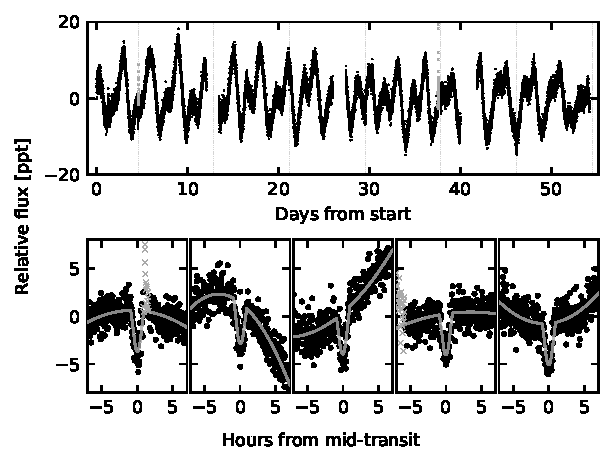
\includegraphics[width=1\textwidth]{f1.pdf}
	\end{center}
	\vspace{-0.7cm}
	\caption{
    {\bf TESS light curve of \tn\ from Sectors 10 and 11.} {\it Top}:
    \texttt{PDCSAP} median-subtracted relative flux at 2-minute
    sampling in units of parts-per-thousand ($\times 10^{-3}$).
    Spot-induced stellar variability is the dominant signal.  Dashed
    lines show the five transits observed by TESS.  {\it Bottom}:
    Zoomed windows of individual transits.  Red points are manually
    identified stellar flares.
		\label{fig:rawzoom}
	}
\end{figure*}

\begin{figure*}[!t]
	\begin{center}
		\leavevmode
		\subfloat{
			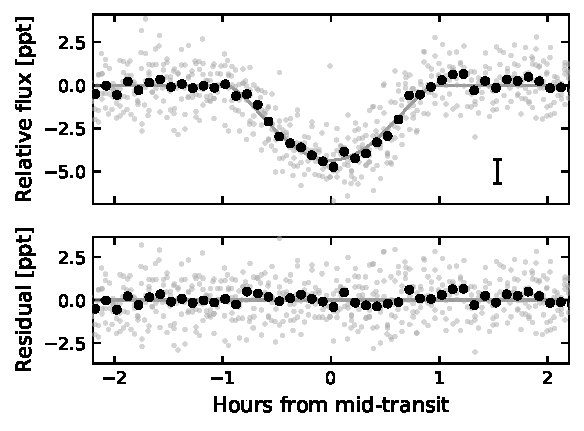
\includegraphics[width=0.8\textwidth]{f2a.pdf}
		}
		
		\vspace{-0.6cm}
		\subfloat{
			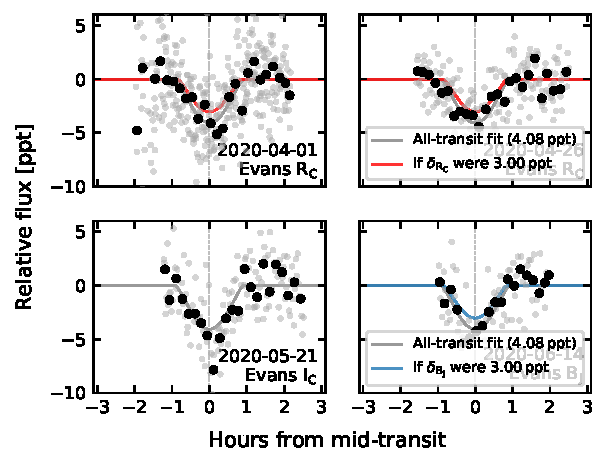
\includegraphics[width=0.8\textwidth]{f2b.pdf}
		}
	\end{center}
	\vspace{-0.7cm}
  \caption{
    {\bf Photometry of \tn.} {\it Top:}
    Phase-folded TESS transit. Gray points are 2-minute PDCSAP flux
    measurements, detrended with a 0.3-day robust Huber spline (see
    Section~\ref{subsec:tess}).  Black points are binned to 6-minute
    intervals.  The gray line shows the median transit model corresponding to the
    fitted to both the TESS and ground-based transits
    (Table~2).  {\it Bottom:} Multicolor
    photometry from the El Sauce 0.36m; gray points are binned to 10-minute intervals.  Models
    show lower limits on the transit depths in 
    the Cousins-R and Johnson-B bandpasses used to rule out specific false positive scenarios.
    \label{fig:jointphot}
	}
\end{figure*}

\tn\ was observed by TESS from 26 March 2019 until 20 May 2019, during
the tenth and eleventh sectors of science operations
\citep{ricker_transiting_2015}.  The star was designated
TIC\,460205581 in the TESS Input Catalog
\citep{stassun_TIC_2018,stassun_TIC8_2019}.  Pixel data for an
$11\times11$ array surrounding the star were averaged and saved at
2-minute cadence.  The $2048\times2048$ image from the entire CCD was
also averaged into 30-minute stacks, and saved as a ``full frame
image'' (FFI).

The TESS project detected the transits in the 2-minute data and the
community was alerted on 17 June 2019.  While our CDIPS FFI light
curves also show the transits, the 2-minute data have better sampling
cadence, and so we opted to use the Presearch Data Conditioning (PDC)
light curve with the default aperture for our
analysis~\citep{smith_kepler_2012,stumpe_multiscale_2014,jenkins_tess_2016,smith_finding_2016}.

Figure~\ref{fig:rawzoom} shows the data.  The dominant modulation
induced by starspots coming into and out of view has a peak-to-peak
amplitude of about 2.3\%, and a period of about 3 days.  The dips
suggestive of a grazing transiting planet recur roughly every 8 days,
and have a depth of about 0.4\%.  A few flares are visible.  A
phase-folded view of the TESS transits with starspot variability
removed is shown in Figure~\ref{fig:jointphot}, and is described in
depth in Section~\ref{subsec:planet}.

%TODO: you must check custom lightkurve apertures, too

%FIXME: this paragraph doesn't really belong here?
We examined the CDIPS FFI light curves of the target, which are
available on MAST \citep{bouma_cluster_2019}. Three light curves are
available, based on photometric apertures with a radius of 1, 1.5, or
2.5 pixels.  In the raw difference-image light-curves, as well as the
PCA-detrended light-curves, dips of depth $\approx$0.35\% are visible,
and their properties do not significantly vary with aperture size.
Within $\approx20$'', the dips are consistent with originating from
the target star.



\subsection{Gaia Astrometry and Imaging}
\label{subsec:gaia}

\begin{figure}[!t]
	\begin{center}
		\leavevmode
		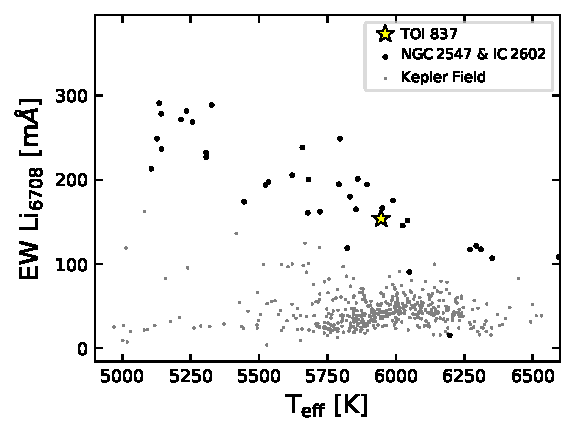
\includegraphics[width=0.45\textwidth]{f5.pdf}
	\end{center}
	\vspace{-0.7cm}
	\caption{ {\bf Scene of \tn.}
    {\it Top:} Mean TESS image of \tn\ over Sector~10, with a
    logarithmic grayscale. The yellow star is the position of \tn.
    Orange circles are neighboring stars with $T<16$ (brighter stars
    are larger). The \texttt{X} and \texttt{/} hatches show the
    apertures used to measure the background and target star flux,
    respectively. Dashed lines of constant declination and right
    ascension are shown.  {\it Bottom:} Digitized Sky Survey $R$-band
    image of the same field, with a linear grayscale.  Two stars of
    interest are ``Star A'' and ``Star B'', which were eventually
    excluded as being possible sources of the transits.
		\label{fig:scene}
	}
\end{figure}

Between 25 July 2014 and 23 May 2016, the ESA Gaia satellite measured
about 300 billion centroid positions of 1{.}6 billion stars.  The
positions, proper motions, and parallaxes of the brighest 1{.}3
billion were calculated for the second data release (DR2)
\citep{gaia_collaboration_gaia_2016,lindegren_gaiasoln_2018,gaia_collaboration_gaia_2018}.
\tn\ was assigned the Gaia DR2 identifier 5251470948229949568, and had
276 ``good'' astrometric observations. Its brightness was measured in
the $G$, $Rp$, and $Bp$ bands of the Radial Velocity Spectrometer
\citep{cropper_gaia_2018,evans_gaia_2018}.  

The Gaia imaging, reduced to its point-source catalog, provides
the initial context for analyzing the TESS data.  Stars brighter than
$T=16$, as queried from the Gaia DR2 source catalog, are shown with
orange circles in Figure~\ref{fig:scene}, overlaid on the DSS2 plates
and TESS image.  Given its galactic latitude of $b=-6^\circ$, it is
not surprising that the field of \tn\ is crowded.  The resolved stars
that were of immediate concern for our false positive analysis were as
follows.
\begin{itemize}
  \item \tn\ $\equiv$ TIC 460205581 ($T=9.9$). The target star.
  \item Star A $\equiv$ TIC 847769574 ($T=14.6$), $2.3$'' west. The
    proper motions and parallax of this star imply it is comoving with
    \tn, though with a physical separation of $6.6\pm 0.1\,{\rm pc}$,
    it may not be bound.
  \item Star B $\equiv$ TIC 460205587 ($T=13.1$), $5.4$'' north.  The
    Gaia parallax implies this is a giant background star.
\end{itemize}
An additional source, TIC 847769581, is $4.9$'' from the target, but
too faint ($T=18.8$) to be the source of the observed transit signal.

The Gaia DR2 data for Star A seems poorly behaved.  While Star A has
$G=15.1$, and $Bp=14.9$, no $Rp$ magnitude is reported.
Correspondingly, no RUWE\footnote{ See the Gaia DPAC technical note
GAIA-C3-TN-LU-LL-124-01,
\url{http://www.rssd.esa.int/doc_fetch.php?id=3757412}, accessed
2020-06-22. } value is available.
% The astrometric reduced $\chi^2$ ($\chi^2 / (N-5)$, for $N$ the number
% of good astrometric observations) seems rather poor, at $8.6$.
We suspect that the photometric failure to produce an $Rp$ magnitude,
as well as its poor astrometric fit, are likely due to blending with
\tn.

At the $\approx1'$ resolution of the TESS data, if either Star A
or Star B were eclipsing binaries, they could be the sources of the
transit signal.  A detailed analysis of ground-based seeing-limited
photometry was necessary to assess and rule out this possibility
(Section~\ref{subsec:groundphot}).


\subsection{High-Resolution Imaging}
\label{subsec:speckle}

\begin{figure}[!t]
	\begin{center}
		\leavevmode
		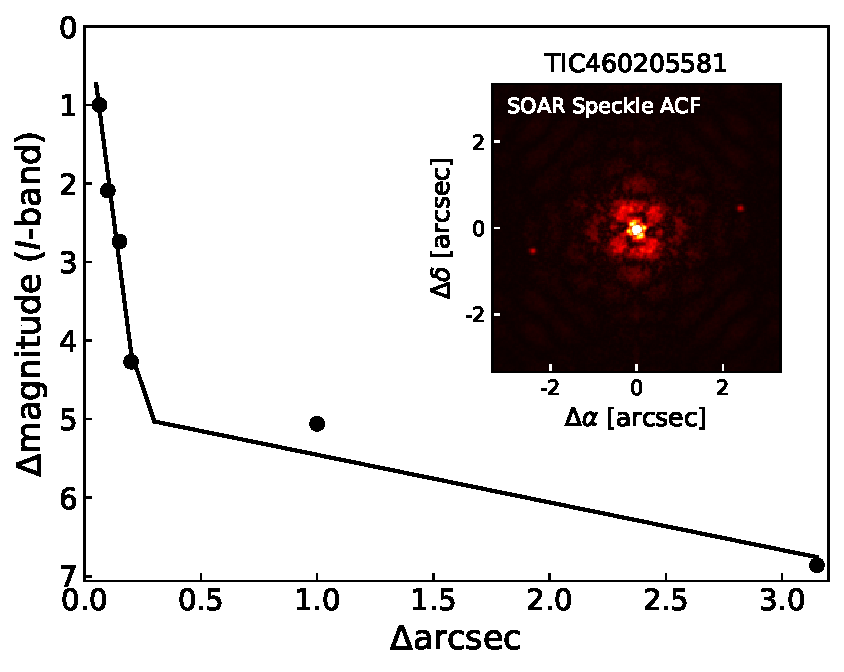
\includegraphics[width=0.45\textwidth]{f6.pdf}
	\end{center}
	\vspace{-0.7cm}
	\caption{ 
    {\bf SOAR HRCam contrast limits derived from point-source
    injection-recovery experiments.} Star A ($\Delta T=4.7$,
    $2.3''$ west) is detected in the autocorrelation function, in
    addition to being a resolved Gaia source.  It is co-moving with
    \tn, and its parallax and on-sky position imply that it is
    physically separated from \tn\ by $6.6\pm 0.1\,{\rm pc}$.
		\label{fig:soar}
	}
\end{figure}

To determine if any fainter point sources existed closer to \tn\
inside of Gaia's point-source detection limits, we acquired
high-resolution speckle images. We then searched the autocorrelation
functions of these images for peaks indicative of nearby companions.

{\bf Carl TODO: please describe and correct as appropriate}
The observations of \tn\ were initially acquired by
\citet{ziegler_soar_2020} as part of the Southern Astrophysical
Research (SOAR) TESS Survey using the High Resolution Camera (HRCam;
\citealt{tokovinin_ten_2018}).  The HRCam $I$-band filter is described
by \citet{tokovinin_ten_2018}.  The points in Figure~\ref{fig:soar}
show the resulting measured 5-$\sigma$ detectable contrasts.  The
lines are linear smoothing fits between the regimes of the diffraction
limit, the ``knee'' at $\approx 0.2''$, and the slow decrease until
$\approx 1.5''$, beyond which the speckle patterns become
de-correlated.  Star A (TIC 847769574) was detected at the expected
location and brightness contrast, and no additional companions were
found.



\subsection{Ground-based Time-Series Photometric Follow-up}
\label{subsec:groundphot}

We obtained ground-based seeing-limited time series photometric
observations of \tn\ bracketed around the times of transit.  These
observations confirmed that the transits occurred on-target to within
$\approx 2''$, and that they were achromatic. Both features are
essential for our ability to eliminate false-positive scenarios.

\subsubsection{El Sauce 0.36m}

\paragraph{Acquisition and reduction}
We observed four transits with the 0.36m at Observatario El Sauce,
located in the R\'io Hurtado Valley in Chile, and operated by
co-author P{.}~Evans.  The observations were obtained in Cousins-R
band on the nights of 1 April 2020 and 26 April 2020, Cousins-I band
on the night of 21 May 2020, and Johnson-B band on the night of 14
June 2020.  The final 14 June transit began shortly after twilight.

{\bf Phil + Karen TODO: please correct as appropriate}
We scheduled the observations using {\bf \texttt{SOFTWARE}} (CITE).
The photometric data were calibrated and extracted using the
\texttt{AstroImageJ} software package
\citep{collins_astroimagej_2017}.  Comparison stars of similar
brightness were used to produce the final light curves, each of which
showed a roughly 4$\,$ppt dip near the expected transit time.


\paragraph{Custom aperture analysis}
Based solely on the TESS data, both Star A and Star B
were possible sources of blended eclipsing binary signals.
For instance, a 30\% eclipse of Star A could produce
dips with the correct depth ($\approx$0.4\%) to explain the \tn\ signal.
Star B is resolved in the ground-based images, while Star A is not.

To assess this possibility with the ground-based photometry, we
produced light curves centered on \tn\ with
circular apertures of radii ranging from 0.7$''$ to 5.1$''$.
We did not detect any statistically significant variation in the depth
of the transits with aperture size.
Two lines evidence rule out Star B as the eclipsing source:
first, the transits
were detected in the smallest apertures.
Second, we made light curves with $2.1''$ apertures centered on Star B,
and they did not show the transit.

To assess the possibility of Star A as the eclipsing body,
we created light curves with a custom set of circular apertures
with radii of $2.1''$ and positions ranging from Star A (2.3$''$ west of \tn) to 2.3$''$
east of \tn.  We did not detect any variation of the transit depth
along this line of light curves, as would be expected if Star A were
the eclipse host.  The apertures east of \tn\ are particularly
constraining, as they exclude over 90\% of the flux from Star A.
The eclipse on Star A would therefore need to be excessively deep to
produce the observed eclipse depth.
We take this as evidence that \tn\ is the source of the transit signal
to within $\approx2.0''$.



\subsubsection{ASTEP400}

{\bf Amaury TODO: please correct as appropriate}
We observed {\bf N} transits with the 0.40m ASTEP 400 telescope at
Concordia Station, located at Dome C on the Antarctic Plateau
\citep{daban_astep_2010}.  ASTEP 400 has a dichroic that sends blue
wavelengths to a guiding camera, and red wavelengths to a filter-free
science camera with wavelength sensitivity roughly akin to R band.
The observations were acquired on the nights of {\bf DATE 1} and {\bf
DATE 2}.  The outdoor temperature was a balmy {\bf XX$^\circ$}.  The
data were reduced using {\bf XX} software, and showed the transit
roughly at the expected time and depth.


\subsection{Spectroscopic Follow-up}
\label{subsec:spectra}

\begin{figure}[!t]
	\begin{center}
		\leavevmode
		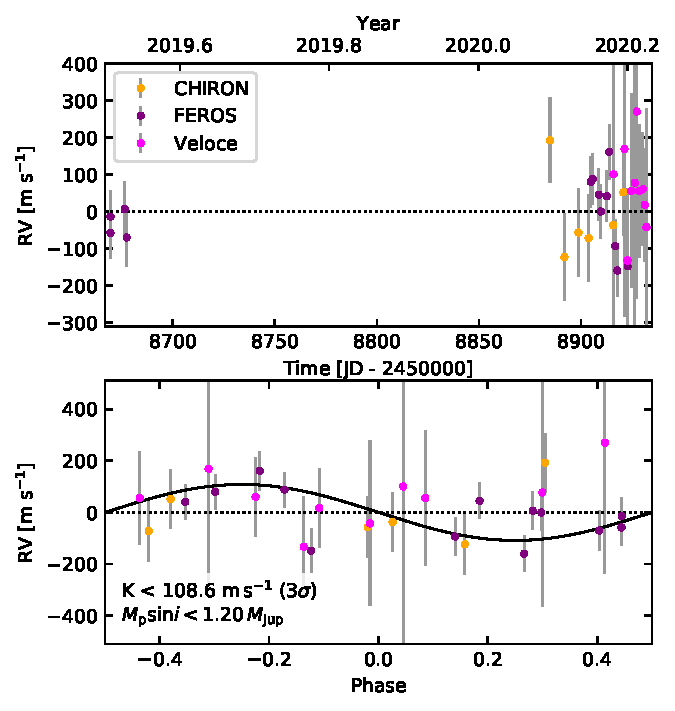
\includegraphics[width=0.48\textwidth]{f3.pdf}
	\end{center}
	\vspace{-0.7cm}
	\caption{
		{\bf Radial velocities of \tn.}
		{\it Top:} RV measurements, with best-fit instrument offsets
    and jitter terms included.  The expected scatter from starspots
    based on $v\sin i$ and the photometric modulation amplitude is of
    order 300m$\,$s$^{-1}$.
		{\it Bottom:}
    RV measurements phased to the orbital ephemeris of \pn.  The
    planet is not detected.  The black line shows a circular
    Keplerian orbit representing the $3\sigma$ upper mass limit.
		\label{fig:rvs}
	}
\end{figure}

Reconaissance spectroscopic follow-up is an essential step in vetting
planet candidates.  Medium to high-resolution spectra enable physical
characterization of the star and therefore planet.  Reducing multiple
spectra to a radial velocity time-series can enable planet mass
measurements, and also set limits on the mass of any nearby
companions.  Finally, if there are close or bright companions,
reconaissance spectra can also reveal the presence of a secondary set
of stellar lines.

\subsubsection{SMARTS 1.5m / CHIRON}
\label{subsec:chiron}

We acquired nine spectra using CHIRON at the SMARTS 1.5m telescope at
Cerro Tollo Inter-American Observatory, Chile
\citep{tokovinin_chironfiber_2013}.  Six met our signal-to-noise
requirements for radial velocity measurements and stellar parameter
extraction.  We used CHIRON in its image slicer configuration,
yielding a spectral resolution of $\approx 79{,}000$ across
415--880$\,$nm.

{\bf George TODO: please describe the formal secondary line search in
more depth in this paragraph} We searched for secondary lines in the
CHIRON spectra by cross-correlating against a {\bf template of some
kind}.  This rules out lines with flux ratios of $\approx 2\%$, if the
lines are well-separated in velocity.  To derive the star's physical
parameters, we cross-correlated the template against {\bf something},
and used the {\bf \texttt{nameofcode}}.  We measured the radial
velocities through a least-squares deconvolution of the observed
spectra against the same synthetic template.  The resulting velocities
are given in Table~\ref{tab:rvs}, and shown in Figure~\ref{fig:rvs}.


\subsubsection{FEROS}
We acquired 13 spectra using the FEROS echelle spectrograph, mounted
on the MPG 2.2m telescope at the European Soutern Observatory in La
Sille, Chile \citep{kaufer_commissioning_1999}.  FEROS has a
resolution of $\approx 48{,}000$ across a spectra range of
350--920$\,$nm. It has a remarkably high efficiency of $\approx 20\%$.

We used the dedicated instrument pipeline to extract 1-dimensional,
wavelength calibrated spectra.  To measure radial velocities, {\bf
Rafael TODO: what procedure was used?  What software packages?}.  The
velocities are given in Table~\ref{tab:rvs}, and shown in
Figure~\ref{fig:rvs}.



\subsubsection{Veloce}
We acquired 34 spectra over 10 visits of \tn\ with using the Veloce
spectrograph, mounted on the AAT 4.0m telescope at Siding Spring
Observatory near Coonabarabran, Australia \citep{gilbert_veloce_2018}.
In Rosso form, Veloce provides coverage from 600--950$\,$nm at a
spectral resolution of $\approx 80{,}000$.

Many of the exposures were taken in average or poor seeing conditions,
when fiber-to-fiber cross-contamination on the IFU-style fiber feed is
strongest.  To reduce the spectra to velocities, we cross-correlated
against a high S/N template of $\delta$ Pavonis.  The velocity RMS
seen across each visit was hundreds of meters per second, likely due to
uncorrected fiber-to-fiber cross-contamination.  For
analysis purposes, we averaged across each visit, and set the velocity
uncertainties to be the standard deviation of the per-visit exposures.
The velocities are given in Table~\ref{tab:rvs}, and shown in
Figure~\ref{fig:rvs}.



\section{Elimination of False Positive Scenarios}
\label{sec:validation}

\begin{figure*}[!t]
	\begin{center}
		\leavevmode
		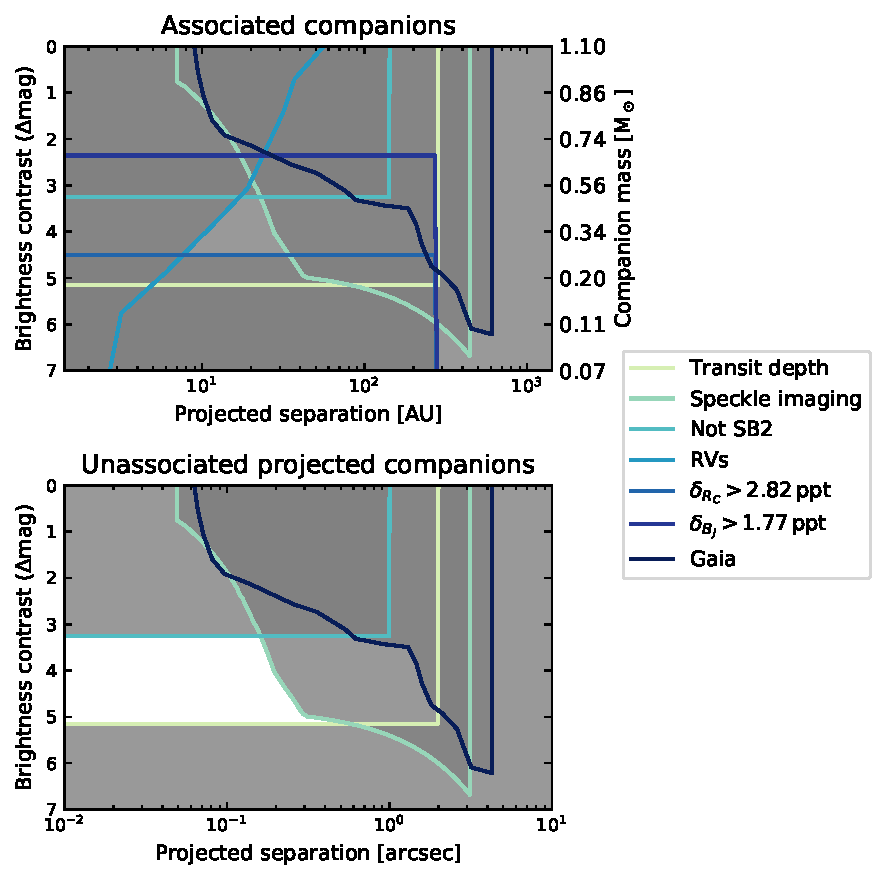
\includegraphics[width=0.85\textwidth]{f4.pdf}
	\end{center}
	\vspace{-0.7cm}
	\caption{
		{\bf Astrophysical false positive scenarios.}
    {\it Top}: for bound companions (EB and HEB scenarios),
		{\it Bottom}: for unassociated companions along the same line of
    sight (BEB scenarios).
		Each constraint is described in Section~\ref{subsec:fp_constraints}.
		\label{fig:fpscenario}
	}
\end{figure*}

Validating a transiting planet means statistically arguing that
the data are much more likely to be caused by a planet than by other
astrophysical false positives. The concept of validation has been
developed and calibrated by {\it e.g.},
\citet{torres_modeling_2011,morton_efficient_2012,diaz_pastis_2014,santerne_pastis_2015,morton_false_2016}
and \citet{giacalone_triceratops_2020}.  ``Validation'' is different
from ``confirmation'', which means that there is overwhelming evidence
that the data must be explained by a planet, for instance through
combined photometric transits and a radial velocity mass measurement.

Assuming the eclipse is localized to the target star, potential false positive scenarios
include eclipses of a background binary (BEB), eclipses of a
hierarchical system bound to the primary star (HEB), and the possibility
that the eclipses are simply caused by a stellar companion,
rather than a planetary one (EB).

Figure~\ref{fig:fpscenario} provides a visual summary of the possible
astrophysical false positive scenarios, as well as our ability to rule
them out based on our combined photometry, velocimetry, and imaging.
We proceed by describing each constraint in detail, and then present a
statistical calculation using \texttt{VESPA}
\citep{morton_efficient_2012} to demonstrate that the probability \tn\
is an astrophysical false positive is small enough to consider it
validated.



\subsection{Constraints on False Positive Scenarios}
\label{subsec:fp_constraints}

\subsubsection{Transit Depth}
In HEB and BEB scenarios, the flux from \tn\ and the true eclipsing
binary host would blend together, reducing the ``true'' eclipse depth
$\delta_{\rm true}$ to produce the observed depth
$\delta_{\rm obs}$:
\begin{equation}
  \delta_{\rm obs}
  = 
  \delta_{\rm true} \frac{F_{\rm neighbor}}{F_{\rm total}},
\end{equation}
where the total flux and the flux from the neighbor are labelled as
such.  The requirement that the eclipse is produced by stars and that
$\delta_{\rm true} < 0.5$ translates to a bound on the faintest
possible blended companion stars:
\begin{equation}
  \Delta m < -\frac{5}{2} \log_{10} \left( \frac{0.5}{\delta_{\rm obs}} \right).
\end{equation}
For \tn\ ($T=9.93$), this implies that any stellar companion invoked
to explain the transit depth must be brighter than $T=15.07$.  In
Figure~\ref{fig:fpscenario}, we set the spatial limit to 2$''$ based
on the precision at which we have localized the transits using
seeing-limited ground-based photometry.

For box-shaped transits, this argument can be
extended to even more restrictive depths \citep[{\it
e.g.},][]{seager_unique_2003,vanderburg_hr858_2019,rizzuto_tess_2020}
However, since the transits of \tn\ are grazing, the second and third
contact points do not occur, and the shape of the transit is not
restrictive.

\subsubsection{Speckle Imaging}
The contrast limits obtained through the SOAR $I$-band speckle imaging
(Section~\ref{subsec:speckle}) are shown in
Figure~\ref{fig:fpscenario}.  While ``Star A'' was detected in the
SOAR images, our ground-based photometry rules it out as a possible
source of the eclipse signal (Section~\ref{subsec:groundphot}).  To
convert the remaining contrast constraints to limits on the masses of
possible bound companions, we used the
\citet{baraffe_evolutionary_2003} models for sub-stellar mass objects
and the MIST isochrones for stellar mass objects
\citep{paxton_modules_2011,paxton_modules_2013,paxton_modules_2015,dotter_mesa_2016,choi_mesa_2016}.
We assumed that the system age was 35 Myr, to ensure that companions
would be at a plausible state of contraction.

To convert from theoretical effective temperatures and bolometric
luminosities to expected magnitudes in instrumental bandpasses, we
assumed that all soruces had blackbody spectra.  While this is
a simplification, the custom instrumental bandpasses prevented a fully
consistent stellar evolutionary calculation.  Using the theoretical
stellar parameters and the measured transmission functions
\citep{tokovinin_ten_2018}, we then calculated the apparent magnitudes
of stellar companions of different masses, and interpolated
to produce the scale shown on the upper-right in
Figure~\ref{fig:fpscenario}.

\subsubsection{Not SB2}
As described in Section~\ref{subsec:chiron}, we searched the CCFs of
the CHIRON spectra to determine whether \tn\ is double-lined.  For a
stellar companion well-separated in velocity, this typically shows
companions with flux-fractions $F_2/F_1 \gtrsim 2\%$.  For plotting
purposes, in Figure~\ref{fig:fpscenario} we have assumed a
flux-fraction limit of 5\% ($\Delta {\rm mag} \approx 3.25$).

\subsubsection{RVs}
The combined radial velocities from FEROS, CHIRON, and Veloce can be
used to place limits on the presence of massive, close-in bound
companion to \tn.  We derived the relevant limits using
\texttt{radvel} \citep{fulton_radvel_2018}.  We assumed circular
orbits for the companion, and then performed two sets of fits.

% timmy.drivers.oneoff_drivers.get_mass_upper_limit
For the first fit, we assumed a restrictive prior on the period and
time of periapse, using the known ephemeris from the transit.  We then
fitted for the period, time of periapse, semi-amplitude, instrument
offsets, and jitter parameters.  This yielded a non-detection of the
planet's orbit.  The corresponding 3-$\sigma$ (99.7$^{\rm th}$
percentile) upper limit on $M_{\rm p} \sin i$ is $1.20 M_{\rm Jup}$.
The data and corresponding model are shown in Figure~\ref{fig:rvs}.

The above exercise rules out the possibility that the observed
eclipses are caused by a star orbiting \tn.  The lack of a linear
trend in the radial velocities, particularly in the FEROS data, can be
used to further limit the presence of a hierarchical binary system.
To constrain this second possibility, we placed a wide log-uniform
prior on the semi-amplitude and period ($\log K\ [{\rm m\,s^{-1}}]
\sim \mathcal{U}(1,10^5)$, $\log P\ [{\rm days}] \sim \mathcal{U}(0.1,
10^{15})$).  We then fitted again for the semi-amplitude, period, time
of conjunction, instrument offsets, and jitter parameters.  We
converted the resulting posterior in period and semi-amplitude to
minimum mass and semi-major axis assuming Kepler's third law.  The
resulting $3\sigma$ limits are shown in Figure~\ref{fig:fpscenario}.

\subsubsection{Multicolor Photometry}
% TODO: this section is ridiculously long. Abbreviate to 2 paragraphs, 3
% at most.

HEB and to a lesser extent BEB scenarios can be limited
by color photometry.
In the absense of color photometry, the most plausible HEB scenarios for TOI
837 involve pairs of eclipsing M dwarfs (Figure~\ref{fig:fpscenario}).
These eclipses are redder than eclipses of the G0V \tn.
Observations that the transit depth does not decrease
going to blue bands can therefore rule out these scenarios.

\paragraph{Simple Example}
% SEE June 1, 2020 email in "Re: TOI-837.01" thread
As a simple example, assume $M_2=M_3=0.2M_\odot$ in a twin HEB.
Assume PMS evolution, and
use MIST isochrones for a 35 Myr system to convert between stellar properties. 
Take transmission functions (filters only; no instrument or atmosphere
response) from the SVO filter profile service\footnote{\url{http://svo2.cab.inta-csic.es/theory/fps/}}.
Integrate up blackbody functions over each bandpass for each star, and
get estimates of the eclipse depths if there were a total eclipse (of
either of the secondary or tertiary) with this set of parameters.  The
apparent eclipse depths in various Bessel and Cousins bandpasses are:
\begin{align}
%FIXME: check these numbers
  \delta_{\rm U_B} &= 5.03\times10^{-4} \ ({\rm Bessel\ U})\nonumber \\
  \delta_{\rm B_B} &= 1.39\times10^{-3}\ ({\rm Bessel\ B})\nonumber \\
  \delta_{\rm V_B} &= 3.31\times10^{-3}\ ({\rm Bessel\ V})\nonumber \\
  \delta_{\rm R_C} &= 5.59\times10^{-3}\ ({\rm Cousins\ R})\nonumber \\
  \delta_{\rm I_C} &= 9.69\times10^{-3}\ ({\rm Cousins\ I})\nonumber \\
  \delta_{\rm T}   &= 9.18\times10^{-3}\ ({\rm TESS})
\end{align}

Our chief interest is the relative depths, because geometry lets all the
depths be scaled to match the observed TESS depth of $\approx$43 ppt.
(In this case, all depths would be scaled down by a multiplicative factor of
2.1).

The crucial point is that the bluest bands--- U and B---are roughly 10
times shallower than TESS-band, because the M dwarf blackbody function
turns over at 2 times longer wavelengths than the G dwarf blackbody
(Wien's law).

Therefore if TOI 837 were a hierarchical eclipsing M dwarf pair,
Phil's two R-band observations should have shown eclipses a factor of
1.64x shallower than TESS observed (so, 24ppt, instead of the ~40ppt
observed). So, the 40 (+/- 10ish) ppt R-band depths seen in Phil's
transits vs TESS-band argue for a planet, but the level of confidence
could probably be improved with U or B.

\paragraph{Limits on Masses of Bound Companions}

With this intuition in place, we derived the limits on masses of bound
hierarchical eclipsing companions as follows.  We assumed that each
system was composed of the primary (\tn), plus a tertiary companion
eclipsing a secondary companion every 8.3 days.

For secondary masses ranging from 0.07 to 1.10 $M_\odot$, and
mass ratios ($M_3/M_2$) from 0.1 to 1, we then 
calculated the observed maximal eclipse depth of Star 3 in front of
Star 2 in a number of bandpasses.
As before, we interpolated between mass, effective temperature, and radius
assuming the MIST isochrones for a 35$\,$Myr old system,
and also assumed that each source had a blackbody spectrum.

We excluded systems for which the maximal eclipse depth in TESS-band
was less than the observed depth ({\it i.e.}, systems for which the tertiary
was too small).
For the systems with maximal eclipse depths in TESS-band greater than
the observed TESS-band depth, we then calculated the multiplicative
factor required to shrink the depth (from the $b=0$ case) to match the
observed eclipse depth in the TESS-band.
We then scaled the depths in each of the other bandpasses by this
fixed geometric factor.

We then asked: given a fixed secondary mass, are there any tertiary
companions for which the expected $\delta_{\rm R_C}$ is larger than
the observed Rc-band depth?
In cases for which the answer was yes, we could not rule out such
hierarchical eclipsing binary systems.
Conversely, we were able to rule out systems
for which at fixed secondary mass no tertiary mass would
enable eclipses (in ${\rm R_C}$-band) of the necessary depth.

For a lower limit on $\delta_{\rm R_C}$ of 30$\,$ppt,
we found that the transition between systems that would produce
eclipses that no matter what were ``too red'', and systems that would
produce eclipses that could be sufficiently blue happens in \tn\ (for
${\rm R_C}$-band) at 0.38$M_\odot$.
The corresponding limit is shown in Figure~\ref{fig:fpscenario}.
For a $\delta_{\rm B_J}$ limit of 30$\,$ppt, the corresponding mass
limit is 0.82$M_\odot$.

\paragraph{Limits on Masses of Projected Companions}

Ignoring the effects of interstellar reddening,
the constraint that $M_2 \gtrsim 0.54 M_\odot$ based on
colors applies to background eclipsing binaries as well.
However, the blue eclipses produced by such systems ({\it e.g.}, a background G2V+K6V binary)
can be kept while making the systems fainter by moving them to greater
distances.
The only way to definitively rule out such scenarios is to 
prove that the loss of light is from the target star,
for instance by detecting the Rossiter-McLaughlin effect
during a transit.

Such scenarios are somewhat contrived in that since 
no secondary eclipse is observed, they require either
eccentric orbits to avoid secondary eclipses, or else a
background twin binary system at double
the orbital period.

\subsubsection{Gaia}

The ``Gaia'' curve in Figure~\ref{fig:fpscenario} combines both
point-source detections from imaging, and sources that show an
astrometric excess.  The curve was interpolated from Figure~4 of
\citet{rizzuto_zeitVIII_2018}.  \tn\ has a RUWE statistic of 1.022,
indicative that there are no obviously present astometric companions.
The UWE statistic (square-root of the reduced astrometric $\chi^2$) is
1.38, which is consistent with stars of similar brightness and color
\citep[][Appendix A]{lindegren_gaiasoln_2018}.

% chi2AL is 526.88
% NgAL is 276
% so, well, reduced chi2 is ~2, which seems bad. but it might (in fact,
% probably is) be because of the color-dependent stuff in the Gaia PSF
% model. Most Rp=10 PTFO members had red chi2 of at least 2.
% Also, looking at Lindegren+2018 Fig A.1., sqrt(reduced chi2) ~= 1.4
% is expected.
%
% --> you could still create the same RUWE vs cluster membership
%  diagnostic plot, just to be sure.


\subsubsection{Patient Imaging}

Archival SERC-J and AAO-SES plates are available for the \tn\
field\footnote{\url{https://archive.stsci.edu/cgi-bin/dss_form}}.
These plates were acquired in 1982 and 1992, respectively.  For high
proper motion stars archival imagery can be used to detect slowly
moving background stars that might be an astrophysical false-positive
source ({\it e.g.}, \citealt{huang_pimen_2018},
\citealt{vanderburg_hr858_2019}).  However \tn\ has only moved
$\approx0.7''$ between 1982 and present, in comparison to the
$\approx2.0''$ FWHM of the target on the plates.  We therefore cannot
resolve it with great confidence from background sources not already
resolved through more modern imaging.


\subsection{False positive probability}

% 151 T<15.1 stars within 360 arcseconds
% 298 T<16.0 stars within 360 arcseconds
The constraints on false-positive scenarios summarized in
Figure~\ref{fig:fpscenario} rule out the possibilities that {\it i)}
the eclipses are caused by a star orbiting \tn, {\it ii)} the eclipses
are caused by hierarchical blends, and {\it iii)} the eclipses are
caused by neighboring stars outside $\approx 2''$.  The only scenario
not formally ruled out is a background eclipsing binary.  A simple
(fallacious) argument on the a priori probability of background blends
follows from counting statistics.  The local density of $T<15.1$ stars
around \tn, found by counting from TIC8, is $3.7\times10^{-4} \,{\rm
arcsec}^{-2}$.  Therefore within the relevant $\approx0.3''$ radius
not excluded by the SOAR HRCam contrast curve, for a randomly selected
star we would expect $1.0\times10^{-4}$ potential $T<15.1$
contaminants, which appears small.

The reason the above statement is an insufficient argument against
BEBs is that \tn\ is not a randomly selected star---it was selected
because it shows eclipses.  Given a foreground star that shows
eclipses, the probability of a background star being present is much
greater than for an arbitrary foreground star.  The relevant
populations need to be modelled at the Monte Carlo level.  We opt to
use \texttt{VESPA} to perform this population modelling
\citep{morton_efficient_2012,vespa_2015}.

\texttt{VESPA} calculates the false positive probability for a transit
signal as
\begin{equation}
  {\rm FPP} = 1 - P_{\rm pl},
\end{equation}
where in our case the probability that the signal comes from a planet,
$P_{\rm pl}$, is given by
\begin{align}
  P_{\rm pl} = 
  \frac{
    \mathcal{L}_{\rm pl}\pi_{\rm pl}
  }{
    \mathcal{L}_{\rm pl}\pi_{\rm pl} + \mathcal{L}_{\rm BEB}\pi_{\rm BEB}
  },
\end{align}
where $\mathcal{L}_i$ is the model likelihood for the planet and BEB
scenarios, and $\pi_i$ is the model prior.  The terms labelled as
``BEB'' usually include other false positive scenarios (HEBs and EBs),
but our followup data have excluded these possibilities.  The priors
are evaluated using a combination of galactic population synthesis
\citep{girardi_star_2005}, binary star statistics
\citep{raghavan_survey_2010}, and specific planet occurrence rates
\citep[][Section~3.4]{morton_efficient_2012}.  The likelihoods are
evaluated by forward-modelling a representative population of
eclipsing bodies for model class, in which each population member has
a particular trapezoidal eclipse depth, total duration, and ingress
duration.  The likelihood is then calculated by multiplying the
probability distribution function of simulated population's shape
parameters with the posterior probability of the actual observed
eclipse shape.

% results from 20200624_simple_fpp_weak_sec 
We ran \texttt{VESPA}\footnote{We used \texttt{VESPA-0.6} and
\texttt{isochrones-1.2.2}.}, and directly incorporated our constraints
of the SOAR $I$-band contrast curve and a non-detection of secondary
eclipses with a depth set at roughly twice the limits from the SPOC
vetting report (0.1\%).  We verified that changing the secondary
eclipse depth limit did not significantly affect the results.  We set
the maximum aperture radius at $2''$, based on our ground-based
photometry.  Incorporating the constraints from
Figure~\ref{fig:fpscenario}, our nominal false positive probability
analysis excluded EB and HEB scenarios.  This yielded a FPP of 0.21\%
for \pn, sufficient for formal validation as a planet
\citep{morton_efficient_2012}.  We did not incorporate our constraint
that \tn\ is not double-lined, which rules out an additional portion
of BEB parameter space.  Had we not acquired multicolor ground-based
photometry, and been unable to exclude HEB scenarios, the FPP would
have risen to 8\%.  However, since the transits are achromatic
(Figure~\ref{fig:jointphot}), particularly in Johnson-B band, we can
rule out HEB scenarios.


\section{System Modelling}
\label{sec:system}

\begin{figure}[!t]
	\begin{center}
		\leavevmode
		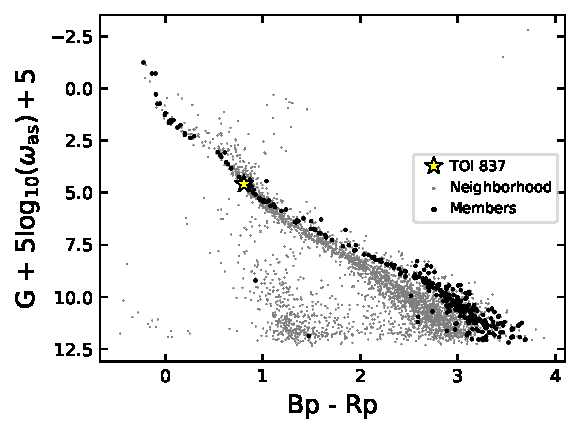
\includegraphics[width=0.45\textwidth]{f7.pdf}
	\end{center}
	\vspace{-0.7cm}
	\caption{ 
  {\bf Hertzsprung-Russell diagram of \tn\ and members of \cn.}
  Members (black circles) were identified by
  \citet{cantatgaudin_gaia_2018}.  Gray circles are non-member stars
  within 5 standard deviations of the mean \cn\ right ascension,
  declination, and parallax.  $G$ denotes Gaia broadband magnitudes,
  $Bp$ Gaia blue, $Rp$ Gaia red, and $\omega_{\rm as}$ the parallax in
  arcseconds. 
  \label{fig:hr}
	}
\end{figure}

\begin{figure*}[!t]
	\begin{center}
		\leavevmode
		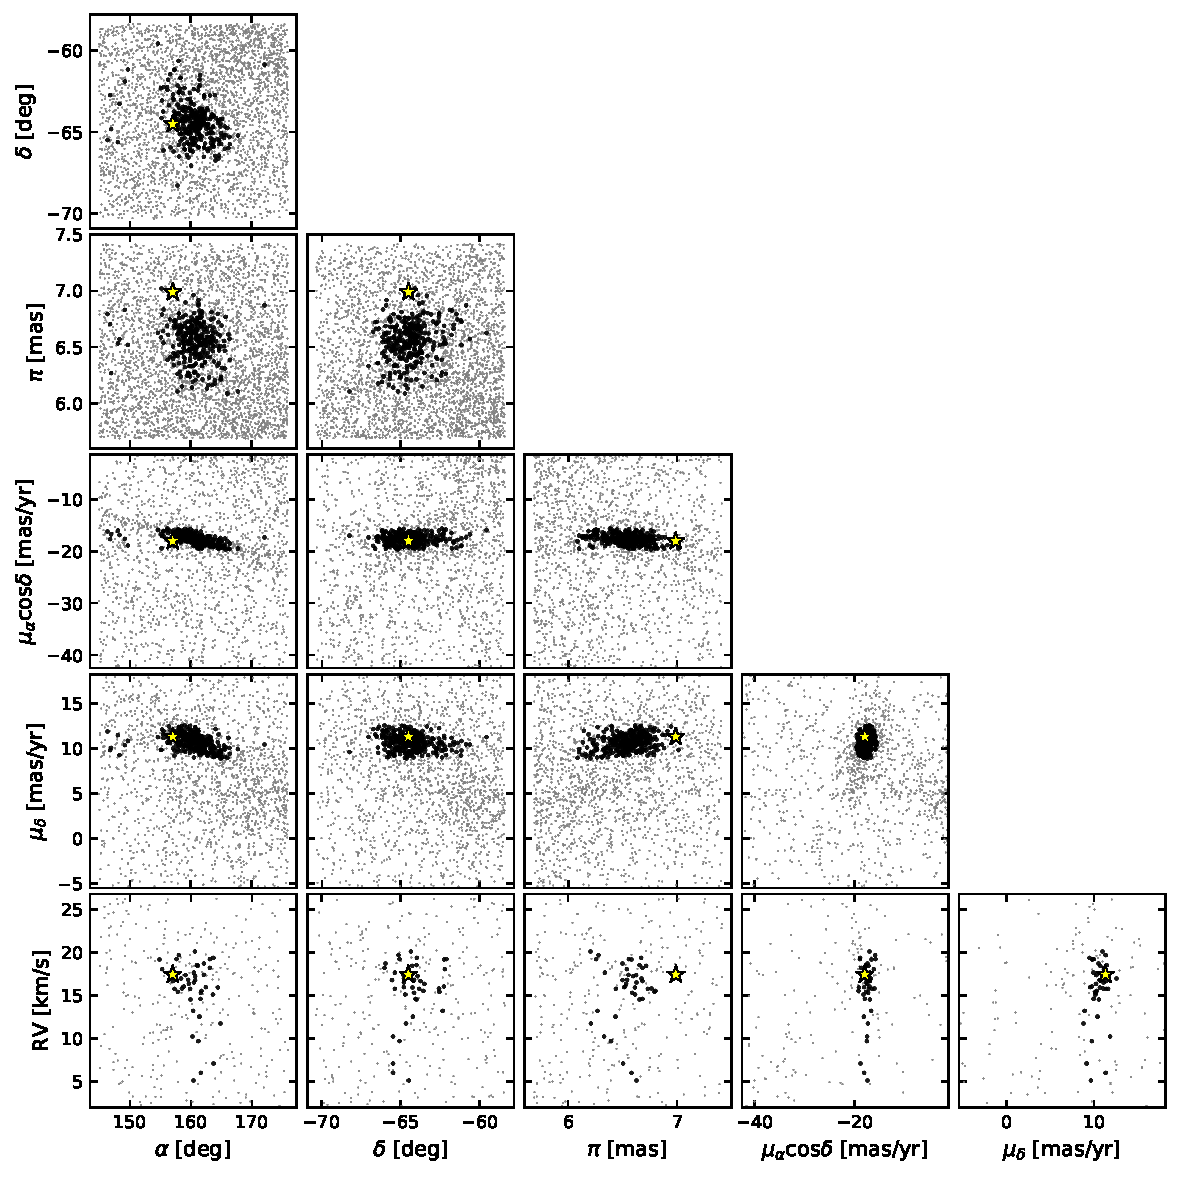
\includegraphics[width=0.7\textwidth]{f8.pdf}
	\end{center}
	\vspace{-0.7cm}
	\caption{ 
  {\bf Positions and kinematics of \tn\ (star), \cn\ members (black
  circles), and stars in the neighborhood (gray circles).} Members
  were identified by \citet{cantatgaudin_gaia_2018}.  $\alpha$ denotes
  right ascension, $\delta$ declination, $\pi$ parallax, $\mu_{\rm
  \delta}$ and $\mu_{\rm \alpha}$ proper motion in each equatorial
  direction, and ${\rm RV}$ radial velocity reported by Gaia DR2.  The
  RVs are for unblended spectra of bright stars ($G\lesssim 12$).  The
  proper motion projection ($\mu_{\delta}$ vs{.} $\mu_{\rm
  \alpha}\cos\delta$) highlights incompleteness in the membership selection function.
  \label{fig:full_kinematics}
	}
\end{figure*}

\begin{figure}[!t]
	\begin{center}
		\leavevmode
		\subfloat{
			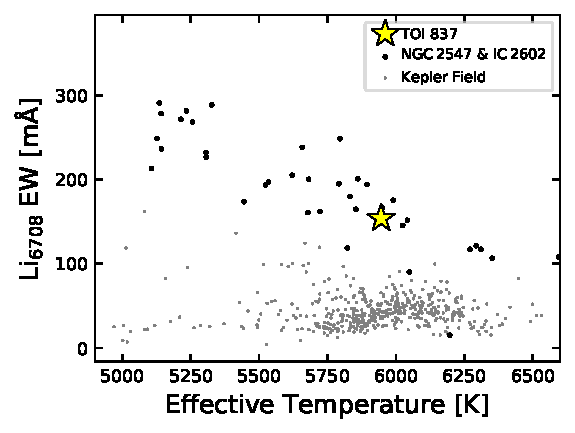
\includegraphics[width=0.45\textwidth]{f9a.pdf}
		}
		
		\vspace{-0.5cm}
		\subfloat{
			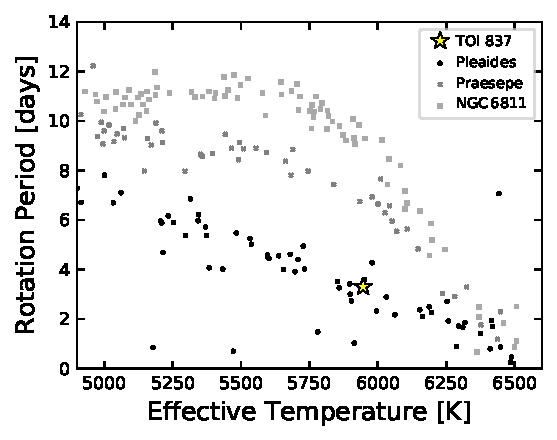
\includegraphics[width=0.45\textwidth]{f9b.pdf}
		}
	\end{center}
	\vspace{-0.7cm}
	\caption{ {\bf Youth diagnostics.}
    {\it Top:} Lithium 6708\AA\ equivalent widths for \tn, field
    stars, and young open clusters.  The field star sample is drawn
    from Kepler planet hosts, and was measured by
    \citet{berger_identifying_2018} using Keck-HIRES.  The young open
    clusters members were surveyed by \citet{randich_gaiaeso_2018}
    using the UVES and GIRAFFE spectrographs at the ESO VLT.
    \citet{randich_gaiaeso_2018} found lithium depletion boundary ages
    for these clusters of $37.7^{+5.7}_{-4.8}\,{\rm Myr}$
    (NGC$\,$2547) and $43.7^{+4.3}_{-3.9}\,{\rm Myr}$ (\cn).  {\it
    Bottom:} Rotation periods for \tn\ and selected open clusters.
    The Pleiades (120$\,$Myr), Praesepe (670$\,$Myr), and NGC$\,$6811
    (1000$\,$Myr) are shown.  Their rotation periods were measured by
    \citet{rebull_rotation_2016a,douglas_poking_2017,douglas_k2_2019},
    and \citet{curtis_temporary_2019}, respectively.
    \label{fig:lithium_rotation}
	}
\end{figure}


%% \begin{deluxetable}{} command tell LaTeX how many columns
%% there are and how to align them.
\begin{deluxetable*}{ccc}
    
%% Keep a portrait orientation

%% Over-ride the default font size
%% Use Default (12pt)
%\tabletypesize{\small}
\tabletypesize{\scriptsize}

%% Use \tablewidth{?pt} to over-ride the default table width.
%% If you are unhappy with the default look at the end of the
%% *.log file to see what the default was set at before adjusting
%% this value.

%% This is the title of the table.
\caption{Previously reported ages for the open cluster IC~2602.}
\label{tab:ages}

%% This command over-rides LaTeX's natural table count
%% and replaces it with this number.  LaTeX will increment 
%% all other tables after this table based on this number
% \tablenum{3}

%% The \tablehead gives provides the column headers.  It
%% is currently set up so that the column labels are on the
%% top line and the units surrounded by ()s are in the 
%% bottom line.  You may add more header information by writing
%% another line between these lines. For each column that requries
%% extra information be sure to include a \colhead{text} command
%% and remember to end any extra lines with \\ and include the 
%% correct number of &s.
\tablehead{\colhead{Method} & \colhead{Age [Myr]} & \colhead{Reference}} 

%% All data must appear between the \startdata and \enddata commands
\startdata
MSTO isochrone & $36.3$ & \citet{mermilliod_comparative_1981} \\
PMS+MSTO isochrone & $30 \pm 5$ & \citet{stauffer_rotational_1997} \\
Isochrone (a) & $67.6$ & \citet{kharchenko_astrophysical_2005} \\
Isochrone (b) & $221$ & \citet{Kharchenko_et_al_2013} \\
Isochrone  & $67.6$ & \citet{van_leeuwen_parallaxes_2009} \\
LDB (c) & $46^{+6}_{-5}$ & \citet{dobbie_ic_2010} \\
MSTO isochrone (d) & $41-46$ & \citet{david_ages_2015} \\
MSTO isochrone (e) & $37-43$ & \citet{david_ages_2015} \\
Li selection + isochrone & $43.7^{+4.3}_{-3.9}$ & \citet{bravi_gaia-eso_2018} \\
Isochrone (f) & $30^{+9}_{-7}$ & \citet{randich_gaiaeso_2018} \\
LDB & $43.7^{+4.3}_{-3.9}$ & \citet{randich_gaiaeso_2018} \\
Isochrone & $35.5^{+0.8}_{-1.6}$ & \citet{bossini_age_2019} \\
Isochrone & $35.5^{+14.6}_{-10.4}$ & \citet{kounkel_untangling_2019} \\
\enddata

%% Include any \tablenotetext{key}{text}, \tablerefs{ref list},
%% or \tablecomments{text} between the \enddata and 
%% \end{deluxetable} commands

%% General table comment marker
\tablecomments{
  MSTO $\equiv$ main sequence turn-off.
  PMS $\equiv$ pre-main-sequence.
	LDB $\equiv$ lithium depletion boundary.
 (a) Based on location in HR diagram of just two stars.
 (b) Notes major age change since \citet{kharchenko_astrophysical_2005}.
 (c)
  \citet{dobbie_ic_2010} performed a dedicated study of the LDB in IC~2602.  Comparing to early isochronal ages, they write their age is ``consistent with the general trend delineated by the Pleiades, $\alpha$-Per, IC$\,$2391, and NGC$\,$2457, whereby the LDB age is ~120-160 per cent of the estimates derived using more traditional techniques'' such as isochrone fitting.
 (d)
  Using \citet{ekstrom_grids_2012} evolutionary models.
 (e)
  Using PARSEC evolutionary models \citep{bressan_parsec_2012}.
 (f)
  Averaged across PROSECCO, PARSEC, MIST models in $(J, H, K_{\rm s})$ and $(J, H, K_{\rm s}, V)$ planes.
} 
\vspace{-1cm}
\end{deluxetable*}


\begin{table}
\scriptsize
\setlength{\tabcolsep}{2pt}
\centering
\caption{Literature and Measured Properties for TOI$\,$837}
\label{tab:starparams}
%\tablenum{2}
\begin{tabular}{llcc}
  \hline
  \hline
Other identifiers\dotfill & \\
\multicolumn{3}{c}{TIC 460205581} \\
\multicolumn{3}{c}{GAIADR2 5251470948229949568} \\
\hline
\hline
Parameter & Description & Value & Source\\
\hline 
$\alpha_{J2015.5}$\dotfill	&Right Ascension (RA)\dotfill & 10:28:08.95 & 1	\\
$\delta_{J2015.5}$\dotfill	&Declination (Dec)\dotfill & -64:30:18.76 & 1	\\
$l_{J2015.5}$\dotfill	&Galactic Longitude\dotfill & 288.2644 & 1	\\
$b_{J2015.5}$\dotfill	&Galactic Latitude\dotfill & -5.7950 & 1	\\
%\\
%$NUV$\dotfill           & GALEX $NUV$ mag.\dotfill & 13.804 $\pm$ 0.004 & 2 \\
%$FUV$\dotfill           & GALEX $FUV$ mag.\dotfill & 18.466 $\pm$ 0.056 & 2 \\
\\
B\dotfill			&Johnson B mag.\dotfill & 11.119 $\pm$ 0.107		& 2	\\
V\dotfill			&Johnson V mag.\dotfill & 10.635 $\pm$ 0.020		& 2	\\
%$B$\tablenote{The uncertainties of the photometry have a systematic error floor applied. Even still, the global fit requires a significant scaling of the uncertainties quoted here to be consistent with our model, suggesting they are still significantly underestimated for one or more of the broad band magnitudes}\dotfill		& APASS Johnson $B$ mag.\dotfill	& 13.001 $\pm$	0.02& 2	\\
%$V$\dotfill		& APASS Johnson $V$ mag.\dotfill	& 11.808 $\pm$	0.02& 2	\\
%\\
${\rm G}$\dotfill     & Gaia $G$ mag.\dotfill     & 10.356$\pm$0.020 & 1\\
${\rm Bp}$\dotfill     & Gaia $Bp$ mag.\dotfill     & 10.695 $\pm$0.020 & 1\\
${\rm Rp}$\dotfill     & Gaia $Rp$ mag.\dotfill     & 9.887$\pm$0.020 & 1\\
${\rm T}$\dotfill     & TESS mag.\dotfill     & 9.9322$\pm$0.006 & 2\\
%$u'$\dotfill        & Sloan $u'$ mag.\dotfill & 14.706 $\pm$ 0.006& 3\\
%$g'$\dotfill		& APASS Sloan $g'$ mag.\dotfill	& 12.407 $\pm$ 0.02	&  2	\\
%$r'$\dotfill		& APASS Sloan $r'$ mag.\dotfill	& 11.311 $\pm$ 0.02	&  2	\\
%$i'$\dotfill		& APASS Sloan $i'$ mag.\dotfill	& 10.927 $\pm$ 0.04 &  2	\\
%\\
J\dotfill			& 2MASS J mag.\dotfill & 9.392  $\pm$ 0.030	& 3	\\
H\dotfill			& 2MASS H mag.\dotfill & 9.108 $\pm$ 0.038	    &  3	\\
K$_{\rm S}$\dotfill			& 2MASS ${\rm K_S}$ mag.\dotfill & 8.933 $\pm$ 0.026 &  3	\\
%\\
W1\dotfill		& WISE1 mag.\dotfill & 8.901 $\pm$ 0.023 & 4	\\
W2\dotfill		& WISE2 mag.\dotfill & 8.875 $\pm$ 0.021 &  4 \\
W3\dotfill		& WISE3 mag.\dotfill &  8.875 $\pm$ 0.020& 4	\\
W4\dotfill		& WISE4 mag.\dotfill & 8.936 $\pm$ N/A &  4	\\
\\
$\pi$\dotfill & Gaia DR2 parallax (mas) \dotfill & 6.989 $\pm$ 0.022 &  1 \\
$d$\dotfill & Distance (pc)\dotfill & $143.1 \pm 0.5$ & 1 \\
$\mu_{\alpha}$\dotfill		& Gaia DR2 proper motion\dotfill & -18.017 $\pm$ 0.039 & 1 \\
                    & \hspace{3pt} in RA (mas yr$^{-1}$)	&  \\
$\mu_{\delta}$\dotfill		& Gaia DR2 proper motion\dotfill 	&  11.307 $\pm$ 0.037 &  1 \\
                    & \hspace{3pt} in DEC (mas yr$^{-1}$) &  \\
RV\dotfill & Systemic radial \hspace{9pt}\dotfill  & $17.44 \pm 0.64$$^{\dagger}$ & 1 \\
                    & \hspace{3pt} velocity (\kms)  & \\
%
\\
$v\sin{i_\star}$\dotfill &  Rotational velocity (\kms) \hspace{9pt}\dotfill &  17.48 $\pm$ 0.15 & 5 \\
${\rm [Fe/H]}$\dotfill &   Metallicity \hspace{9pt}\dotfill & -0.065 $\pm$ 0.035 & 5 \\
$T_{\rm eff}$\dotfill &  Effective Temperature (K) \hspace{9pt}\dotfill & 6047 $\pm$ 40  &  6  \\
$\log{g_{\star}}$\dotfill &  Surface Gravity (cgs)\hspace{9pt}\dotfill &  4.467 $\pm$ 0.010  &  6 \\
%
Li EW\dotfill & 6708\AA\ Equiv{.} Width (m\AA) \dotfill & $154 \pm 9$  & 7 \\
%
$P_{\rm rot}$\dotfill & Rotation period (d)\dotfill & $3.004\pm 0.053$  & 8 \\
Age & Adopted stellar age (Myr)\dotfill & $30$--$46$  &  9 \\
% $E(B-V)$\dotfill & Reddening (mag)\dotfill & $0.06 \pm 0.02$ & 9 \\
%
Spec. Type\dotfill & Spectral Type\dotfill & 	G0V & 5 \\
%
$R_\star$\dotfill & Stellar radius ($R_\odot$)\dotfill & 1.022$\pm$0.015 & 6 \\
$M_\star$\dotfill & Stellar mass ($R_\odot$)\dotfill & 1.118$\pm$0.011 & 6 \\
%$F_{\rm bol}$\dotfill & Stellar bolometric flux (cgs)\dotfill & (1.967$\pm$0.046)$\times10^{-9}$ & 9 \\
$A_{\rm V}$\dotfill & Interstellar reddening (mag)\dotfill & 0.20$\pm$0.03 & 10 \\
% $U^{*}$\dotfill & Space Velocity (\kms)\dotfill & $26.24 \pm 0.46$  & \S\ref{sec:uvw} \\
% $V$\dotfill       & Space Velocity (\kms)\dotfill & $-71.52 \pm 1.68$ & \S\ref{sec:uvw} \\
% $W$\dotfill       & Space Velocity (\kms)\dotfill & $ -1.31 \pm 0.27$ & \S\ref{sec:uvw} \\
\hline
\end{tabular}
\begin{flushleft}
 \footnotesize{ \textsc{NOTE}---
$\dagger$ Systemic RV uncertainty is the standard deviation of single-transit radial velocities, as quoted in Gaia DR2. %$*$ $U$ is in the direction of the Galactic center. \\
Provenances are:
$^1$\citet{gaia_collaboration_gaia_2018},
$^2$\citet{stassun_TIC8_2019},
$^3$\citet{skrutskie_tmass_2006},
$^4$\citet{wright_WISE_2010},
$^5$CHIRON spectra,
$^6$Method~2 (cluster isochrone, Section~\ref{subsec:starparams}),
$^7$FEROS spectra,
$^8$TESS light curve,
$^9$IC~2602 ages from isochrone \& lithium depletion analyses (Section~\ref{subsec:clusterchar}),
$^10$Method~1 (photometric SED fit, Section~\ref{subsec:starparams}).}
\end{flushleft}
\vspace{-0.5cm}
\end{table}


% Table of best fit parameters
%\startlongtable
\begin{deluxetable*}{lllrrrrr}
%
  \tablecaption{ Priors and posteriors for the model fitted to the
  TESS data.}
\label{tab:posterior}
%
%\tabletypesize{\scriptsize}
%
%\tablenum{2}
%
\tablehead{
  \colhead{Param.} & 
  \colhead{Unit} &
  \colhead{Prior} & 
  \colhead{Median} & 
  \colhead{Mean} & 
  \colhead{Std{.} Dev.} &
  \colhead{3\%} &
  \colhead{97\%}
}

% /Users/luke/Dropbox/proj/timmy/results/TOI_837_tessindivtransit_phot_results/20200711/posterior_table_clean_tessindivtransit.tex
\startdata
$P$ & d & $\mathcal{N}(8.3249; 0.1000)$ & 8.3247158 & 8.3247141 & 0.0003210 & 8.3240946 & 8.3253007 \\
$t_0^{(1)}$ & d & $\mathcal{N}(1574.273800; 0.1000)$ & 1574.2730012 & 1574.2730125 & 0.0010420 & 1574.2710233 & 1574.2749496 \\
$\log R_{\rm p}/R_\star$ & -- & $\mathcal{U}(-4.605; 0.000)$ & -2.51877 & -2.50605 & 0.09466 & -2.66494 & -2.32807 \\
$b$ & -- & $\mathcal{U}(0; 1+R_{\mathrm{p}}/R_\star)$ & 0.9521 & 0.9536 & 0.0125 & 0.9318 & 0.9768 \\
$u_1$ & -- & $\mathcal{U}(0.175; 0.475)$$^{(2)}$ & 0.335 & 0.332 & 0.086 & 0.196 & 0.475 \\
$u_2$ & -- & $\mathcal{U}(0.085; 0.385)$$^{(2)}$ & 0.243 & 0.240 & 0.086 & 0.105 & 0.384 \\
$R_\star$ & $R_\odot$ & $\mathcal{T}(1.022; 0.015)$ & 1.022 & 1.022 & 0.015 & 0.994 & 1.050 \\
$\log g$ & cgs & $\mathcal{N}(4.467; 0.010)$ & 4.467 & 4.467 & 0.010 & 4.448 & 4.486 \\
$a_{00;\mathrm{TESS}}$ & -- & $\mathcal{N}(1.00; 0.01)$ & 0.9985 & 0.9985 & 0.0001 & 0.9983 & 0.9986 \\
$a_{01;\mathrm{TESS}}$ & d$^{-1}$ & $\mathcal{U}(-0.05; 0.05)$ & -0.0004 & -0.0004 & 0.0003 & -0.0011 & 0.0002 \\
$a_{02;\mathrm{TESS}}$ & d$^{-2}$ & $\mathcal{U}(-0.05; 0.05)$ & -0.0168 & -0.0168 & 0.0023 & -0.0211 & -0.0124 \\
$a_{10;\mathrm{TESS}}$ & -- & $\mathcal{N}(1.00; 0.01)$ & 1.0089 & 1.0089 & 0.0001 & 1.0088 & 1.0091 \\
$a_{11;\mathrm{TESS}}$ & d$^{-1}$ & $\mathcal{U}(-0.05; 0.05)$ & -0.0138 & -0.0138 & 0.0003 & -0.0144 & -0.0132 \\
$a_{12;\mathrm{TESS}}$ & d$^{-2}$ & $\mathcal{U}(-0.05; 0.05)$ & -0.0536 & -0.0536 & 0.0022 & -0.0577 & -0.0494 \\
$a_{20;\mathrm{TESS}}$ & -- & $\mathcal{N}(1.00; 0.01)$ & 0.9991 & 0.9991 & 0.0001 & 0.9989 & 0.9993 \\
$a_{21;\mathrm{TESS}}$ & d$^{-1}$ & $\mathcal{U}(-0.05; 0.05)$ & 0.0156 & 0.0156 & 0.0004 & 0.0150 & 0.0163 \\
$a_{22;\mathrm{TESS}}$ & d$^{-2}$ & $\mathcal{U}(-0.05; 0.05)$ & 0.0246 & 0.0246 & 0.0024 & 0.02 & 0.0289 \\
$a_{30;\mathrm{TESS}}$ & -- & $\mathcal{N}(1.00; 0.01)$ & 1.0012 & 1.0012 & 0.0001 & 1.0010 & 1.0014 \\
$a_{31;\mathrm{TESS}}$ & d$^{-1}$ & $\mathcal{U}(-0.05; 0.05)$ & 0.0021 & 0.0021 & 0.0004 & 0.0014 & 0.0029 \\
$a_{32;\mathrm{TESS}}$ & d$^{-2}$ & $\mathcal{U}(-0.05; 0.05)$ & -0.0079 & -0.0079 & 0.0029 & -0.0133 & -0.0025 \\
$a_{40;\mathrm{TESS}}$ & -- & $\mathcal{N}(1.00; 0.01)$ & 0.9906 & 0.9906 & 0.0001 & 0.9904 & 0.9907 \\
$a_{41;\mathrm{TESS}}$ & d$^{-1}$ & $\mathcal{U}(-0.05; 0.05)$ & 0.0015 & 0.0015 & 0.0003 & 0.0009 & 0.0022 \\
$a_{42;\mathrm{TESS}}$ & d$^{-2}$ & $\mathcal{U}(-0.05; 0.05)$ & 0.0327 & 0.0327 & 0.0023 & 0.0283 & 0.0370 \\
$R_{\rm p}/R_\star$ & -- & -- & 0.08 & 0.08 & 0.01 & 0.07 & 0.10 \\
$\rho_\star$ & g$\ $cm$^{-3}$ & -- & 1.47 & 1.47 & 0.04 & 1.40 & 1.55 \\
$R_{\rm p}$ & $R_{\mathrm{Jup}}$ & -- & 0.80 & 0.82 & 0.08 & 0.68 & 0.97 \\
$a/R_\star$ & -- & -- & 17.54 & 17.54 & 0.16 & 17.24 & 17.84 \\
$\cos i$ & -- & -- & 0.05 & 0.05 & 0. & 0.05 & 0.06 \\
$T_{14}$ & hr & -- & 1.85 & 1.86 & 0.04 & 1.78 & 1.93 \\
$T_{13}$ & hr & -- & 0.20 & 0.21 & 0.10 & 0.01 & NaN$^{(3)}$ \\
\enddata
%
\tablecomments{
(1) For the most precise ephemeris based on the combination of TESS and
ground-based data, please see Equation~\ref{eq:ephem}; the period and epoch are noted
in this table only for self-consistency.
%
% (2) Uninformative quadratic limb-darkening prior from \citet{exoplanet:kipping13}, implemented by \citet{exoplanet:exoplanet}.
% The precision achieved in the ground-based data did not appear to
% necessitate using bandpass-dependent limb-darkening coefficients.
% For comparison, the \citet{claret_limb_2017} parameters for
% the appropriate $T_{\rm eff}$ and $\log g$ in TESS-band would have been 
% $(u_1, u_2) = (0.3249, 0.235)$.
%
(2) Assuming an informative quadratic limb-darkening prior with
values about those given for the appropriate $T_{\rm eff}$ and
$\log g$ in TESS-band from \citet{claret_limb_2017}. The precision
achieved in the ground-based data did not appear to necessitate using
bandpass-dependent limb-darkening coefficients.
(3) The second and third contact points do not exist for a grazing transit.
{\it Notation}:
$a_{ij;\mathrm{Instr}}$ denotes the $i^{\rm th}$ transit of a
particular instrument, and the $j^{\rm th}$ polynomial detrending
order.
$\mathcal{U}$ denotes a uniform distribution,
$\mathcal{N}$ a normal distribution, and
$\mathcal{T}$ a truncated normal bounded between zero and an upper limit much larger than the mean.
}
\vspace{-0.3cm}
\end{deluxetable*}



\subsection{The Cluster}
\label{subsec:cluster}

\subsubsection{Physical Characteristics}
\label{subsec:clusterchar}

The \cn\ cluster is about 150$\,$pc from the Earth, and is near the
galactic plane with $(l,b)\approx(289.6^\circ, -5.0^\circ)$
\citep{cantatgaudin_gaia_2018}.  It is also sometimes called the
$\theta$ Carinae cluster, after its brightest member.  While \cn\ is
close to the Lower Centaurus Crux subgroup of the Scorpio-Centaurus
OB2 association in both position and proper motion space, its older
age and clear kinematic separation indicate that it is a distinct
stellar population
\citep{de_zeeuw_hipparcos_1999,damiani_stellar_2019}.

Reliable ages reported for \cn\ range from 30--46$\,$Myr.  We have
collected ages reported over the years in Table~\ref{tab:ages}.  The
Li depletion boundary technique yields slightly older absolute ages
than isochrone fitting \citep{dobbie_ic_2010,randich_gaiaeso_2018}.
Rather than redetermine the age of the cluster and add another line to
the table, we simply adopt the absolute age range for \tn\ of
30--46$\,$Myr.

Reported mean metallicity values ${\rm [Fe/H]}$ for the cluster range
between slightly super-solar ($0.04\pm0.01$,
\citealt{baratella_gaia-eso_2020}) and slightly sub-solar ($-0.02 \pm
0.02$, \citealt{netopil_metallicity_2016}).  The extinction $E(B-V)$
is rather low, with reported values ranging from 0.03 to 0.07
\citep[{\it e.g.},][]{randich_gaiaeso_2018}.

Kinematically, IC~2602 seems to be supervirial, in the sense that the
observed stellar velocity dispersion is larger than the value expected
if it were in virial equilibrium by about a factor of two
\citep{bravi_gaia-eso_2018}.  \citet{damiani_stellar_2019} also
reported evidence for the ongoing evaporation of \cn, in the form of a
diffuse $\approx10^\circ$ halo of young stars around the central
density cusps.  A gyrochronological study of these stars could confirm
that these stars are truly coeval with the cluster.

\subsubsection{HR Diagram}

Figure~\ref{fig:hr} shows a Hertzsprung-Russell diagram of \tn, the
\cn\ cluster, and the ``neighborhood'' of spatially nearby stars.
Stars labelled as ``cluster members'' are those reported by
\citet{cantatgaudin_gaia_2018} based on Gaia DR2 positions, proper
motions, and parallaxes.  We included candidate members with formal
membership probability exceeding 10\%.  Save for a few low-mass
outliers, most members appear to be young and coeval.

\tn\ is in its expected position relative to the other members along
the cluster isochrone.  This photometrically limits the presence of
binary companions in the \tn\ system, to within perhaps half the
brightness ($\approx0.75$ magnitudes) of the target star.

Figure~\ref{fig:hr} also suggests that the membership census of \cn\
is incomplete.  We defined the reference ``neighborhood'' as the group
of at most $10^4$ randomly selected non-member stars within 5 standard
deviations of the mean \cn\ right ascension, declination, and
parallax.  We queried Gaia DR2 for these stars using
\texttt{astroquery} \citep{astroquery_2018}.  Many low-mass stars
appear above the main sequence, even though they were not identified
as 5-dimensional kinematic members through the unsupervised
\citet{cantatgaudin_gaia_2018} membership assignment process.


\subsection{The Star}
\label{subsec:star}

\subsubsection{Membership of \tn\ in \cn}
\label{subsec:member}

\tn\ has been reported as a member of \cn\ by many independent
investigators \citep[{\it
e.g.},][]{Kharchenko_et_al_2013,oh_comoving_2017,cantatgaudin_gaia_2018,damiani_stellar_2019,kounkel_untangling_2019}.
The simplest way to verify the membership is through inspection of the
Gaia DR2 position and kinematics.  Figure~\ref{fig:full_kinematics}
shows the six-dimensional positions and kinematics of \tn, \cn\
members, and nearby stars.  The ``neighborhood'' is defined as in
Figure~\ref{fig:hr}.  The axes limits for the right ascension,
declination, and parallax dimensions are set by being within 5
standard deviations of the mean \cn\ right ascension, declination, and
parallax.  The axes limits for the proper motion and radial velocity
dimensions are set at the 25$^{\rm th}$ and 75$^{\rm th}$ percentiles,
in order to give a sense of the population's distribution, while
excluding outliers.  The radial velocities suffer the greatest
incompleteness due to the current $G\approx12$ magnitude limit of the
Gaia DR2 data processing.

Figure~\ref{fig:full_kinematics} provides strong evidence that \tn\ is
a member of \cn.  The only dimension that could lead to some worry is
the parallax, as \tn\ is one of the closest \cn\ members reported by
\citet{cantatgaudin_gaia_2018}.  Fortunately, there are independent
means of verifying the star's youth.

\subsubsection{Rotation}

As stars get older, their rotation rates incrementally slow due to
magnetic braking \cite{weber_angular_1967,skumanich_time_1972}.  One
way to verify the youth of \tn\ is by comparing its rotation period to
other stars with known ages.

We measured the rotation period from the PDCSAP light curve using the
Lomb-Scargle periodogram implemented in \texttt{astropy}
\citep{lomb_1976,scargle_studies_1982,vanderplas_periodograms_2015}.
We fitted the light curve without masking out the transits or flares,
as these represent a small fraction of the overall time series.  To
derive the uncertainty on the best period, we fitted a gaussian to the
dominant peak, after first ensuring that we had oversampled the
initial frequency grid.  This gave a rotation period of $P_{\rm rot} =
2.987 \pm 0.056\,{\rm d}$ when allowing for a single Fourier terms in
the periodogram model, and $P_{\rm rot} = 3.004 \pm 0.053\,{\rm d}$
when allowing for two Fourier terms.  As the second model provides a
better fit to the data, we adopt the second measurement.

As we will discuss in Section~\ref{subsec:starparams}, we measured the
star's radius by combining the spectroscopic effective temperature
with a broadband photometry SED fit.  We would expect, combining our
$R_\star$ and $P_{\rm rot}$ measurements, that the equatorial velocity
$v$ of the star would be $17.67 \pm 0.32 \,{\rm km\,s}^{-1}$.  Our
spectroscopically measured $v\sin i$ from CHIRON, $17.48 \pm 0.15
\,{\rm km\,s}^{-1}$ agrees reasonably well with this expectation.

The star is clearly a rapid rotator.
Figure~\ref{fig:lithium_rotation} compares its rotation period with
rotation periods that have been measured in a number of well-studied
open clusters.  \tn\ seems to be gyrochronologically coeval with the
Pleiades sequence.  This is not to say that \tn\ is ``Pleaides-aged'',
because the observed scatter in the rotation-period diagram for the
first 10--100$\,$Myr is quite high \citep[see Figure~9
of][]{rebull_rotation_2020}.  Instead, we interpret the rotation
period as evidence to support the claim that \tn\ is younger than $\sim$
$500\,{\rm Myr}$.


\subsubsection{Lithium}

Lithium depletion for early G-dwarfs like \tn\ requires hundreds of
megayears \citep{soderblom_ages_2014}. This is because their
convective envelopes are shallow, and so transport of photospheric
lithium to the hot core takes place over diffusive timescales, rather
than convective timescales.  Nonetheless, comparison of early G-dwarfs
in the field to {\it e.g.}, 600 Myr old Hyads has shown that the
depletion does indeed happen over many gigayears
\citep{berger_identifying_2018}.

The spectra of \tn\ all show the 6708$\,$\AA\ lithium doublet in
absorption. Opting to use our FEROS spectra because of their high S/N,
we measured the line's equivalent width (EW) to be $154 \pm 9 \,
$m\AA.  Figure~\ref{fig:lithium_rotation} compares this EW to stars in
the field, and other young open cluster members.  The field star
measurements were collected by \citet{berger_identifying_2018}; we
show their reported lithium detections with ${\rm S/N}>3$.  The young
open cluster members were selected for the presence of lithium, as
described by \citet{randich_gaiaeso_2018}.  The measured \tn\ Li EW is
much larger than observed for field stars, and is consistent with
lithium absorption seen in stars with similar colors in sub-100$\,{\rm
Myr}$ moving groups.


\subsubsection{Stellar Parameters}
\label{subsec:starparams}

Select properties of \tn\ from the literature and our analysis are
presented in Table~\ref{tab:starparams}.  The spectroscopic parameters
were measured from each of the six CHIRON spectra
(Section~\ref{subsec:chiron}). We then averaged the results, and
adopted the standard deviation across the spectra as the uncertainty.

We then calculated the stellar radius and reddening following
\citet{stassun_accurate_2017}.  We first derived the bolometric flux
by combining available broadband magnitudes from Gaia, Tycho-2, APASS,
2MASS, and WISE.  We then fitted the SED with the
\citet{kurucz_atlas12_2013} stellar atmopshere models, and summed to
find $F_{\rm bol}$.  When fitting the atmosphere model, we varied the
extinction ($A_{\rm V}$) and the overall normalization.  This
procedure yielded $A_{\rm V} = 0.20\pm0.03$, which independently
agrees with the average from the \cn\ isochrone fits of
\citet{randich_gaiaeso_2018}.
We then combined the spectroscopic effective temperature, bolometric
flux, and Gaia distance to determine the stellar radius, using the
Stefan-Boltzmann law.


\subsection{The Planet}
\label{subsec:planet}

To derive physical parameters of \pn\ based on the photometry, we
fitted the TESS and ground-based transits simultaneously.

\subsubsection{Transit Fitting}
Simultaneous dip plus rotation period (GP) fit. Use celerite plus PyMC3/exoplanet.
Mention FPP?

%TODO: describe 0.3-day robust Huber spline (or whatever detrending is
%eventually used)

\subsubsection{Comments on Joint Transit and Radial Velocity Fitting}

The available data for \tn\ put us in an odd position. The transit
data provide a minimum size due to the grazing geometry; the radial
velocity data provide a maximum mass ($\approx$1.20 $M_{\rm jup}$).
We could combine the two with an empirically-calibrated planetary
mass-radius relation to force a more restrictive upper bound on the
planetary size \citep[{\it e.g.},][]{chen_probabilistic_2016}.  The
result of such an exercise would tautologically be that the planet
would be smaller than the largest known Jovian planets ($\approx
2R_{\rm Jup}$).  This would also imply that the impact parameter is
slightly below unity.  The planet's size, in our eyes, would remain
poorly constrained even if we were to do this exercise. {\bf So we
don't do it.}


\subsubsection{Additional Transits}
None of the extra dips in the PDCSAP light-curve (e.g., ``up-down''
spikes at BTJD 1572 and 1601) seem likely to be planetary
We checked that i) they were not present in the SAPFLUX light-curves,
and ii) that they were not present in the CDIPS light-curves (either
raw, or PCA-detrended).

To make this quantitative, we did injection-recovery.



\section{Discussion}
\label{sec:discussion}

\tn\ joins a number of other young planetary systems reported from
TESS, including DS~Tuc~Ab, HIP~67522b, TOI~1726, and AU~Mic~b
\citep{newton_tess_2019,zhou_well_2019,montet_young_2019,rizzuto_tess_2020,mann_tess_2020,plavchan_planet_2020,palle_transmission_2020,addison_youngest_2020,martioli_magnetism_2020,hirano_limits_2020}
However, unlike these planets, \pn\ is validated but not yet confirmed.

The easiest path towards definitively confirming
whether \tn\ is a planet will be a Rossiter-McLaughlin (RM) measurement.  
Detection of the RM signal
would rule out BEB and HEB scenarios, as it would imply that the
eclipsing object is bound to the target star. Combined with our
non-detection of the planet's mass from radial velocity monitoring,
this would confirm that \pn\ is a planet.

The maximum amplitude of the Rossiter-McLaughlin anomaly is
\citep{winn_exoplanet_2010}
\begin{equation}
  \Delta V_{\rm RM} \approx \delta \cdot v\sin i \cdot \sqrt{1-b^2}
  \approx 21\,{\rm m\,s}^{-1},
\end{equation}
where we have assumed stellar and transit parameters from
Tables~\ref{tab:starparams} and~\ref{tab:posterior}, and for
calculation purposes we assumed $b=0.95$.  This is challenging, but
for a 1.9$\,$hr transit of a $V=10.6$ star, a detection could be achieved
with modern spectrographs.  The next viable total transit windows from
Chile occur in January and February of 2021; there are also a few
visible per season from other southern locations.

The Rossiter-McLaughlin approach is more likely to yield short-term
success than a direct mass measurement because of the RV noise
expected to be induced by stellar rotation.  The photometric amplitude
induced by starspots on \tn\ is $\approx 2\%$. 
The RV noise expected over the course of the $\approx 3\,{\rm d}$
rotation period can then be estimated by multiplying the photometric amplitude and
spectroscopic equatorial velocity.  This gives $\sigma_{\rm RV,rot}
\approx 300\,{\rm m\,s}^{-1}$, and is consistent with the scatter we
observe in our radial velocities from FEROS.  Detecting
a planet's Doppler signal in these regimes is
challenging, and requires a significant amount of data and care in
signal extraction \citep{barragan_radial_2019}.  The
Rossiter-McLaughlin measurement avoids the majority of this issue
because the transit occurs over a much shorter duration than a single
stellar rotation period.  

If the RM measurements prove that the planet
is real, a campaign to measure the mass timed to coincide with
TESS sectors 36 and 37 ({\it i.e.}, from late March to late May of
2021) would significantly ease the extraction of the planetary Doppler
signal.  The reason is that the radial velocities, activity
indicators, and photometry could then be fit simultaneously, which
would greatly constrain any gaussian process model for the
spot-induced RV signal. 




%%%%%%%%%%%%%%%%%%%%%%%%%%%%%%%%%%%%%%%%%%%%%%%%%%%%%%%%%%%%%%%%%%%%%%%%%%%%%%%

\acknowledgements
%
%This paper includes data collected by the TESS mission, which are
%publicly available from the Mikulski Archive for Space Telescopes
%(MAST).
%
%Funding for the TESS mission is provided by NASA's Science Mission
%directorate.
%
The authors thank...
%
We also thank the Heising-Simons Foundation for
their generous support of this work.
%
The Digitized Sky Survey was produced at the Space Telescope Science
Institute under U.S. Government grant NAG W-2166.
Figure~\ref{fig:scene} is based on photographic data obtained using
the Oschin Schmidt Telescope on Palomar Mountain.
%
This research made use of the Exoplanet Follow-up Observation
Program website, which is operated by the California Institute of
Technology, under contract with the National Aeronautics and Space
Administration under the Exoplanet Exploration Program.
%
This research has made use of the SVO Filter Profile Service
(\url{http://svo2.cab.inta-csic.es/theory/fps/}) supported from the Spanish
MINECO through grant AYA2017-84089
%
\tn\ was included on the TESS ``short-cadence'' target list in part
thanks to the Guest Investigator program of G.\ Sacco (G011265).

%
% %
% Based on observations obtained at the Gemini Observatory, which is
% operated by the Association of Universities for Research in Astronomy,
% Inc., under a cooperative agreement with the NSF on behalf of the
% Gemini partnership: the National Science Foundation (United States),
% National Research Council (Canada), CONICYT (Chile), Ministerio de
% Ciencia, Tecnolog\'{i}a e Innovaci\'{o}n Productiva (Argentina),
% Minist\'{e}rio da Ci\^{e}ncia, Tecnologia e Inova\c{c}\~{a}o (Brazil),
% and Korea Astronomy and Space Science Institute (Republic of Korea).
% %
% Observations in the paper made use of the High-Resolution Imaging
% instrument Zorro at Gemini-South. Zorro was funded by the NASA
% Exoplanet Exploration Program and built at the NASA Ames Research
% Center by Steve B. Howell, Nic Scott, Elliott P. Horch, and Emmett
% Quigley.
% %
% This research has made use of the VizieR catalogue access tool, CDS,
% Strasbourg, France. The original description of the VizieR service was
% published in A\&AS 143, 23.
% %
% This work has made use of data from the European Space Agency (ESA)
% mission {\it Gaia} (\url{https://www.cosmos.esa.int/gaia}), processed
% by the {\it Gaia} Data Processing and Analysis Consortium (DPAC,
% \url{https://www.cosmos.esa.int/web/gaia/dpac/consortium}). Funding
% for the DPAC has been provided by national institutions, in particular
% the institutions participating in the {\it Gaia} Multilateral
% Agreement.
%
% (Some of) The data presented herein were obtained at the W. M. Keck
% Observatory, which is operated as a scientific partnership among the
% California Institute of Technology, the University of California and
% the National Aeronautics and Space Administration. The Observatory was
% made possible by the generous financial support of the W. M. Keck
% Foundation.
% The authors wish to recognize and acknowledge the very significant
% cultural role and reverence that the summit of Maunakea has always had
% within the indigenous Hawaiian community.  We are most fortunate to
% have the opportunity to conduct observations from this mountain.
%
% \newline
%

\software{
  \texttt{astrobase} \citep{bhatti_astrobase_2018},
  %\texttt{astroplan} \citep{astroplan2018},
	\texttt{AstroImageJ} \citep{collins_astroimagej_2017},
  \texttt{astropy} \citep{astropy_2018},
  \texttt{astroquery} \citep{astroquery_2018},
  %\texttt{BATMAN} \citep{kreidberg_batman_2015},
  \texttt{cdips-pipeline} \citep{bhatti_cdips-pipeline_2019}
  \texttt{corner} \citep{corner_2016},
  %\texttt{emcee} \citep{foreman-mackey_emcee_2013},
  \texttt{exoplanet} \citep{exoplanet:agol19}
  \texttt{exoplanet} \citep{exoplanet:exoplanet}, and its
  dependencies \citep{exoplanet:agol19, exoplanet:kipping13, exoplanet:luger18,
  	exoplanet:theano}.
  \texttt{IPython} \citep{perez_2007},
	\texttt{isochrones} \citep{morton_2015_isochrones},
	\texttt{lightkurve} \citep{lightkurve_2018},
  \texttt{matplotlib} \citep{hunter_matplotlib_2007}, 
  \texttt{MESA} \citep{paxton_modules_2011,paxton_modules_2013,paxton_modules_2015}
  \texttt{numpy} \citep{walt_numpy_2011}, 
  \texttt{pandas} \citep{mckinney-proc-scipy-2010},
  \texttt{pyGAM} \citep{serven_pygam_2018_1476122},
  \texttt{PyMC3} \citep{salvatier_2016_PyMC3},
  \texttt{radvel} \citep{fulton_radvel_2018},
  %\texttt{scikit-learn} \citep{scikit-learn},
  \texttt{scipy} \citep{jones_scipy_2001},
  \texttt{tesscut} \citep{brasseur_astrocut_2019},
	\texttt{VESPA} \citep{morton_efficient_2012,vespa_2015},
  \texttt{webplotdigitzer} \citep{rohatgi_2019},
  \texttt{wotan} \citep{hippke_wotan_2019}.
}


\facilities{
 	{\it Astrometry}:
 	Gaia \citep{gaia_collaboration_gaia_2016,gaia_collaboration_gaia_2018}.
 	{\it Imaging}:
    Second Generation Digitized Sky Survey,
    SOAR~(HRCam; \citealt{tokovinin_ten_2018}).
 	%Keck:II~(NIRC2; \url{www2.keck.hawaii.edu/inst/nirc2}).
 	%Gemini:South~(Zorro; \citealt{scott_nessi_2018}.
 	{\it Spectroscopy}:
	CTIO1.5m~(CHIRON; \citealt{tokovinin_chironfiber_2013}),
    MPG2.2m~(FEROS; \citealt{kaufer_commissioning_1999}),
	AAT~(Veloce; \citealt{gilbert_veloce_2018}).
 	%Keck:I~(HIRES; \citealt{vogt_hires_1994}).
 	%{\bf VLT (number), UVES and GIRAFFE} (CITE: Pasquini et al 2002)
% 	Euler1.2m~(CORALIE),
% 	ESO:3.6m~(HARPS; \citealt{mayor_setting_2003}).
 	{\it Photometry}:
% 	CTIO:1.0m (Y4KCam),
% 	Danish 1.54m Telescope,
	  El Sauce:0.356m,
% 	Elizabeth 1.0m at SAAO,
% 	Euler1.2m (EulerCam),
% 	Magellan:Baade (MagIC),
% 	Max Planck:2.2m	(GROND; \citealt{greiner_grond7-channel_2008})
% 	NTT,
% 	SOAR (SOI),
 	TESS \citep{ricker_transiting_2015}.
% 	TRAPPIST \citep{jehin_trappist_2011},
% 	VLT:Antu (FORS2).
}

%
% The following are entries from Table 1 that are not otherwise cited
% in the text
%
% \nocite{wilson_wasp-4b_2008}
% \nocite{gillon_improved_2009}
% \nocite{winn_transit_2009}
% \nocite{hoyer_tramos_2013}
% \nocite{dragomir_terms_2011}
% \nocite{sanchis-ojeda_starspots_2011}
% \nocite{nikolov_wasp-4b_2012}
% \nocite{ranjan_atmospheric_2014}
% \nocite{huitson_gemini_2017}

% \input{WASP-4b_transit_time_table.tex}
% \input{WASP-4b_rv_table.tex}
% \input{model_fit_table.tex}
% \input{rv_model_posterior_table.tex}
% \input{pdot_table.tex}

\clearpage
%% \begin{deluxetable}{} command tell LaTeX how many columns
%% there are and how to align them.
\startlongtable
\begin{deluxetable*}{cccc}
    
%% Keep a portrait orientation

%% Over-ride the default font size
%% Use Default (12pt)
\tabletypesize{\scriptsize}

%% Use \tablewidth{?pt} to over-ride the default table width.
%% If you are unhappy with the default look at the end of the
%% *.log file to see what the default was set at before adjusting
%% this value.

%% This is the title of the table.
\tablecaption{\tn\ photometry.}
\label{tab:phot}

%% This command over-rides LaTeX's natural table count
%% and replaces it with this number.  LaTeX will increment 
%% all other tables after this table based on this number
\tablenum{3}

%% The \tablehead gives provides the column headers.  It
%% is currently set up so that the column labels are on the
%% top line and the units surrounded by ()s are in the 
%% bottom line.  You may add more header information by writing
%% another line between these lines. For each column that requries
%% extra information be sure to include a \colhead{text} command
%% and remember to end any extra lines with \\ and include the 
%% correct number of &s.
\tablehead{
  \colhead{Time [BJD$_\mathrm{TDB}$]} &
  \colhead{Rel{.} Flux} &
  \colhead{Rel{.} Flux Err{.}} & 
  \colhead{Instrument}
}

%% All data must appear between the \startdata and \enddata commands
% XXX pasted in from selected_transit_times.tex
\startdata
 2451234.12345 &      1.00 &   0.01 &       TESS \\
\enddata

%% Include any \tablenotetext{key}{text}, \tablerefs{ref list},
%% or \tablecomments{text} between the \enddata and 
%% \end{deluxetable} commands

%% General table comment marker
\tablecomments{
Table~1 is published in its entirety in a machine-readable format.
The first entry is shown for guidance regarding form and
content.
}
\vspace{-0.9cm}
\end{deluxetable*}

%% \begin{deluxetable}{} command tell LaTeX how many columns
%% there are and how to align them.
\startlongtable
\begin{deluxetable*}{llll}
    
%% Keep a portrait orientation

%% Over-ride the default font size
%% Use Default (12pt)
\tabletypesize{\scriptsize}

%% Use \tablewidth{?pt} to over-ride the default table width.
%% If you are unhappy with the default look at the end of the
%% *.log file to see what the default was set at before adjusting
%% this value.

%% This is the title of the table.
\tablecaption{\tn\ radial velocities.}
\label{tab:rvs}

%% This command over-rides LaTeX's natural table count
%% and replaces it with this number.  LaTeX will increment 
%% all other tables after this table based on this number
%\tablenum{4}

%% The \tablehead gives provides the column headers.  It
%% is currently set up so that the column labels are on the
%% top line and the units surrounded by ()s are in the 
%% bottom line.  You may add more header information by writing
%% another line between these lines. For each column that requries
%% extra information be sure to include a \colhead{text} command
%% and remember to end any extra lines with \\ and include the 
%% correct number of &s.
\tablehead{
  \colhead{Time [BJD$_\mathrm{TDB}$]} &
  \colhead{RV [m$\,$s$^{-1}$]} &
  \colhead{$\sigma_{\rm RV}$ [m$\,$s$^{-1}$]} & 
  \colhead{Instrument}
}

%% All data must appear between the \startdata and \enddata commands
% Source:
% /Users/luke/Dropbox/proj/timmy/results/paper_tables/TOI837_rv_data.tex
\startdata
 8669.533150 &  -57.80 &   27.50 &   FEROS \\
 8669.540450 &  -13.90 &   29.40 &   FEROS \\
 8676.506930 &    6.70 &   37.80 &   FEROS \\
 8677.519150 &  -70.30 &   44.60 &   FEROS \\
 8884.787630 &  240.00 &   28.00 &  CHIRON \\
 8891.891180 &  -76.00 &   37.00 &  CHIRON \\
 8898.735330 &  -10.00 &   43.00 &  CHIRON \\
 8903.725760 &  -25.00 &   38.00 &  CHIRON \\
 8904.739930 &   80.10 &   24.50 &   FEROS \\
 8905.793630 &   88.00 &   21.70 &   FEROS \\
 8908.762520 &   45.30 &   28.30 &   FEROS \\
 8909.702140 &    0.00 &   31.80 &   FEROS \\
 8912.606750 &   41.30 &   24.10 &   FEROS \\
 8913.740580 &  161.10 &   37.30 &   FEROS \\
 8915.762170 &   10.00 &   33.00 &  CHIRON \\
 8916.714540 &  -93.50 &   33.60 &   FEROS \\
 8917.765720 & -159.70 &   24.80 &   FEROS \\
 8920.706100 &   99.00 &   32.00 &  CHIRON \\
 8922.845800 & -148.30 &   54.90 &   FEROS \\
 8915.924027 &   37.51 &  725.91 &  Veloce \\
 8921.284950 &  105.90 &  453.19 &  Veloce \\
 8922.733572 & -195.92 &  195.63 &  Veloce \\
 8924.583708 &   -7.65 &  262.32 &  Veloce \\
 8926.365810 &   14.28 &  442.64 &  Veloce \\
 8927.318146 &  207.04 &  505.19 &  Veloce \\
 8928.559780 &   -7.28 &  180.24 &  Veloce \\
 8930.324059 &   -2.60 &  152.02 &  Veloce \\
 8931.293091 &  -45.68 &  152.94 &  Veloce \\
 8932.065206 & -105.60 &  319.82 &  Veloce \\
\enddata

%% Include any \tablenotetext{key}{text}, \tablerefs{ref list},
%% or \tablecomments{text} between the \enddata and 
%% \end{deluxetable} commands

%% General table comment marker
\tablecomments{
Times are in units of ${\rm BJD}_{\rm TDB} - 2{,}450{,}000$.
}
\vspace{-0.9cm}
\end{deluxetable*}

%\startlongtable
\begin{deluxetable*}{lrrrrrrrr}
%
%\tabletypesize{\scriptsize}
%
\tablenum{1}
%
\tablecaption{Model Comparison.}
\label{tab:modelcompare}
%
\tablehead{
\colhead{Description} &
\colhead{$N_{\rm s}$} &
\colhead{$N_{\rm \ell}$} &
\colhead{$N_{\rm data}$} &
\colhead{$N_{\rm param}$} &
\colhead{$\chi^2$} &
\colhead{$\chi_{\rm red}^2$} &
\colhead{BIC} &
\colhead{$\Delta$BIC}
}
% pasted from
% /Users/luke/Dropbox/proj/billy/results/PTFO_8-8695_results/20200428_v0/bic_table_data.tex
% 
% Burnham and Anderson 2004.
% "Models having i ≤ 2 have substantial support (evidence), those in which 4 ≤
% i ≤ 7 have considerably less support, and models having i > 10 have
% essentially no support"
\startdata
Favored    & 2 &  2 &   2585 &      17 &  3230.2 &     1.258 &  3363.7 &     0.0 \\
\hline
Weakly favored &  3 &  3 &   2585 &      21 &  3203.4 &     1.249 &  3368.4 &     4.7 \\
---               & 3 &  2 &   2585 &      19 &  3222.9 &     1.256 &  3372.2 &     8.4 \\
\hline
Disfavored      & 2 &  3 &   2585 &      19 &  3244.9 &     1.265 &  3394.2 &    30.4 \\
---              & 2 &  1 &   2585 &      15 &  3410.6 &     1.327 &  3528.5 &   164.7 \\
---             &  3 &  1 &   2585 &      17 &  3396.4 &     1.323 &  3530.0 &   166.3 \\
---             & 1 &  2 &   2585 &      15 &  4158.6 &     1.618 &  4276.4 &   912.7 \\
---             & 1 &  3 &   2585 &      17 &  4147.4 &     1.615 &  4281.0 &   917.2 \\
---            &  1 &  1 &   2585 &      13 &  4313.5 &     1.677 &  4415.6 &  1051.9 \\
\enddata
%
\tablecomments{
	$N_{\rm s}$ and $N_{\rm \ell}$ are the number of harmonics at the short and long periods, respectively.
	$N_{\rm data}$ is the number of fitted flux measurements.
	$N_{\rm param}$ is the number of free parameters in the model.
	The Bayesian information criterion (BIC) and the difference from the maximum $\Delta {\rm BIC}$ are also listed.
}
\vspace{-1cm}
\end{deluxetable*}

\clearpage

\bibliographystyle{yahapj}                            
\bibliography{bibliography} 

% \appendix
% \section{Gaia query}
% bounding by 5 stdevns
% Launched query: '
%         select top 10000
%             g.source_id, g.phot_bp_mean_mag, g.phot_rp_mean_mag,
%             g.phot_g_mean_mag, g.parallax, g.ra, g.dec, g.pmra, g.pmdec,
%             g.radial_velocity, g.radial_velocity_error
%         from gaiadr2.gaia_source as g
%         where
%             g.parallax > 5.69
%         and
%             g.parallax < 7.41
%         and
%             g.dec < -58.41
%         and
%             g.dec > -70.33
%         and
%             g.ra > 145.01
%         and
%             g.ra < 175.85
%         and
%             g.phot_g_mean_mag < 18
%         order by
%             random_index

\listofchanges

\end{document}
